\documentclass[11pt]{article}
\usepackage[margin=1in]{geometry}
\usepackage{graphicx}
\usepackage{fancyhdr}
\usepackage{titling}
\usepackage{enumitem}
\usepackage{hyperref}
\usepackage{xcolor}
\usepackage{amsmath}
\usepackage{booktabs}
\usepackage{caption}
\usepackage{tabularx}
\usepackage[most]{tcolorbox}
\usepackage{float}

\setlength{\headheight}{40pt}
\setlength{\headsep}{20pt}

\hypersetup{
  colorlinks=true,
  urlcolor=blue,
  linkcolor=black,
  citecolor=black,
  pdfborder={0 0 0},
}

\pagestyle{fancy}
\fancyhf{}
\lhead{
\includegraphics[height=1.4cm]{logo.png}}
\rhead{\small \textsf{Schmidt Sciences \\ Astrophysics Institute}}
\cfoot{\thepage}

\pretitle{\vspace{1cm}\begin{center}\LARGE\bfseries}
\posttitle{\par\end{center}\vskip 1.5em}
\preauthor{\begin{center}\large\lineskip 0.5em%
    \begin{tabular}[t]{c}}
\postauthor{\end{tabular}\end{center}}
\predate{\begin{center}\large}
\postdate{\end{center}}

\newcommand{\docidprefix}{SM\_00X\_Lazuli}
\newcommand{\observatory}{Lazuli}

\title{\observatory\ Science Memo: Cross-checking the \texttt{lazuli-exo} IFS Transmission-Spectroscopy Simulator Against As-Measured Data}
\author{G.~Stefansson \\}
\date{5 October 2026}

\begin{document}

\maketitle
\thispagestyle{fancy}

\begin{center}
\begin{tcolorbox}[colback=gray!10!white, colframe=gray!50!black,
                  boxrule=0.5pt, width=0.9\textwidth]
\centering
\textbf{Content marked for:} \textcolor{red}{\textbf{Internal Only}} / \textcolor{teal}{External Use}
\end{tcolorbox}
\end{center}

\begin{center}
\textbf{Document ID:} \texttt{\docidprefix}
\end{center}

\vspace{1em}
\noindent
\textbf{Document Version History}
\vspace{0.5em}

\begin{tabular}{|p{1.5cm}|p{2.5cm}|p{3cm}|p{4cm}|p{4cm}|}
\hline
\textbf{Version} & \textbf{Date} & \textbf{Authors} & \textbf{Change Description} & \textbf{Approved By / Date} \\
\hline
0.1 & 2026-09-26 & GS (drafted with Claude Code) & Initial draft; pilot checks A and B run & \\
\hline
0.2 & 2026-10-05 & GS (drafted with Claude Code) & Checks A--D and G run; see ``Changes since v0.1'' & \\
\hline
\end{tabular}

\vspace{1.5em}

% ============================================================================
\section*{Summary of decisions}

\texttt{lazuli-exo} predicts Lazuli IFS transmission spectra and error bars for 14 showcase planets (POSEIDON tables) and for any planet (parametric model, \texttt{lazuli\_exo.simulate}). Version 0.1 of this memo defined eight cross-checks against \emph{as-measured} data and ran two pilots, one of which found the Vega/AB magnitude bug. That bug is fixed and the noise tables were regenerated on 2026-10-04. This version runs checks A--D and G against public archives and published JWST and HST data. All numbers below are derived here unless marked otherwise; scripts and data snapshots are in \texttt{memo/scripts/} and \texttt{memo/data/}.

\begin{itemize}[leftmargin=*]
  \item \textbf{The photon-normalization chain is now exactly right (check B(i)).} The v0.1 pilot found that slicersim normalized the 2MASS $J$ (Vega) magnitudes as AB, making every host 2.3$\times$ too bright; that is fixed. An independent hand budget $F_\lambda\,\lambda/(hc)\,A\,\eta\,{\rm QE}\,\Delta\lambda\,t_{\rm int}$, normalized to the catalog $J$ with sncosmo, reproduces slicersim's extracted signal to $1.000$ for all 14 hosts at every wavelength (Table~B1). The Vega/AB fix is confirmed end to end.
  \item \textbf{Against JWST, Lazuli's predicted errors are consistent with collecting-area scaling (check B(ii)).} For WASP-39\,b, lazuli-exo predicts a single-transit precision 2.3$\times$ worse than NIRISS/SOSS achieved in the same 0.004\,$\mu$m bins, against 1.9$\times$ from area alone; for NIRSpec/PRISM it predicts 1.2$\times$ worse (Table~B2). Against 23 of 27 HST datasets Lazuli predicts errors 0.07--0.66$\times$ the published values, well below the 0.80 area ratio (Figure~2): HST's duty cycle and systematics, and in some cases several combined transits, set those. Lazuli's statistical-only bars are a photon floor, not a forecast.
  \item \textbf{Stellar SEDs pass for hot hosts, not for M dwarfs (check A).} $J$-normalized model flux over Gaia DR3 XP flux is within 10\,\% at 0.40--1.02\,$\mu$m for seven of the eight hosts hotter than 4400\,K; WASP-12 (6265\,K) is 1.2$\times$ in the blue. The star tables over-predict the blue flux of GJ~1214 by 1.40$\times$ and GJ~3470 by 1.20$\times$. The parametric path's PHOENIX mini-grid has corrupt nodes at non-solar metallicity below 3500\,K: LHS~1140 comes out 0.63$\times$ XP in the blue (GitHub \#16, new).
  \item \textbf{The registry is not self-consistent for two targets (check C).} $t_{14}$ recomputed from the registry's own geometry is 0.85$\times$ the registry $t_{14}$ for HAT-P-11\,b and 0.93$\times$ for LHS~1140\,b; all other targets agree within 3.5\,\%. For the eleven targets with two or more published solutions and $\Delta k/k\ge1$\,\%, the white-light depths differ by 140--1900\,ppm between references (HD~209458\,b: 34\,ppm), against a Lazuli single-transit white-light depth error of 2--25\,ppm. The transit solver matches batman to 0.07\,ppm; the local-arc $z(t)$ is off by up to 69\,ppm (WASP-12\,b).
  \item \textbf{The clear H$_2$/He scenario over-predicts every measured spectrum (check D).} Fitting data $= c + b\times$model, the clear scenario gives $b \le 0.69$ for all 33 space-based datasets with at least 10 points, and $b<0$ for seven of them (two WASP-12\,b, five of six TRAPPIST-1\,e; Table~D1, Figure~3). The scenario set brackets the measured amplitude for 23 of 47 datasets on the table path and 31 of 47 on the parametric path (15 and 22 of the 35 space-based ones). TRAPPIST-1\,e's four JWST visits are flat ($b_{\rm clear}\le 0.08$); WASP-107\,b is nearly flat ($b_{\rm clear}=0.09$). The reduced $\chi^2$ of the nearest toy scenario against JWST-quality data is 5--6.
  \item \textbf{Stellar contamination is measurable and already matters for TRAPPIST-1\,e (check G).} The four JWST/PRISM visits scatter by 220\,ppm visit to visit at 1.0--1.7\,$\mu$m, of which 180\,ppm is in excess of the per-visit errors, and their mean depths differ by 430\,ppm. Lazuli's single-transit error there is 330\,ppm per channel, so after about three transits the unmodelled stellar term dominates (GitHub \#8).
  \item \textbf{Not run:} E (fitted limb darkening), F (H4RG lab ramps) and H (slicersim time-series injection). E needs fitted coefficients that are not tabulated in the archive; F and H need internal inputs.
  \item \textbf{Decisions.} (0) Fix TRAPPIST-1\,e's limb-darkening table, which has six chunks with negative limb intensity at 0.41--0.74\,$\mu$m (GitHub \#10). (1) Present ``clear'' as an upper envelope and make ``cloudy'' or ``high metallicity'' the default showcase scenario for sub-Neptunes; drop the H$_2$/He scenarios for TRAPPIST-1\,e and LHS~1140\,b. (2) Fix the PHOENIX mini-grid (\#16) and normalize the M-dwarf showcase stars to Gaia XP. (3) Freeze one solution per target (\#7). (4) Add a stellar-contamination term bounded by check G before quoting any M-dwarf S/N (\#8). (5) Keep the ``statistical noise only'' caveat; the HST comparison shows why.
\end{itemize}

\noindent\textbf{Changes since v0.1.} Checks A, B, C, D and G run on the regenerated (Vega/AB-corrected) noise tables and on the parametric path; package renamed \texttt{lazuli-exo}; JWST data added (WASP-39\,b NIRISS and PRISM, TRAPPIST-1\,e four PRISM visits); references verified against arXiv abstracts; checks E, F, H not run. Corrected: WASP-107 $\Delta(V{-}J)$ from $+0.27$ to $+0.09$ (SIMBAD $V$ now 11.47). After an internal review of the figures on 2026-10-05: all four figures redrawn (data and Lazuli error bars at the same bins, clear and cloudy scenarios as the two brackets), $A_{\rm HST}$ set to the geometric 4.52\,m$^2$, the single-transit white-light depth error added to Table~C2, ``best'' renamed ``nearest toy'', and three Summary statements corrected against the tables (checks A, C, D).

% ============================================================================
\section*{Background}

\texttt{lazuli-exo} (formerly \texttt{terminator}) is a numpy-only runtime over precomputed tables: POSEIDON isothermal equilibrium-chemistry H$_2$/He scenarios for 14 planets, slicersim single-transit noise tables for the \texttt{lazuli\_cbe} configuration, exotic-ld limb-darkening tables, and, since 2026-10-04, a planet-independent photospheric-pressure grid and a PHOENIX stellar mini-grid that let \texttt{simulate()} model any planet with slicersim computing the noise live. Target parameters are frozen from the NASA Exoplanet Archive composite table.

Version 0.1 of this memo argued that every validation to date was internal and proposed eight as-measured checks. Its pilot photon budget found that 2MASS $J$ (Vega) was normalized as AB inside slicersim, making every host 2.3$\times$ too bright. That was fixed in \texttt{lazuli\_exo.slicer.depth\_error} and the noise tables were regenerated against slicersim 1.0.0 (\texttt{0947b53}). The 2026-10-05 review (\texttt{report/2026-10-05\_report.md}) then found that the two model paths disagree with each other by 5--75\,\% in feature amplitude for the same planet because of the 10-bar reference-radius convention of the tables (GitHub \#3). The checks below therefore test both paths wherever a model spectrum enters.

% ============================================================================
\section*{Modeling Approach}

Each check isolates one stage of the forward model and compares it with a measured quantity. Throughout: model products come from the committed tables and the committed grids, never regenerated ad hoc; all scripts run in the \texttt{py313} environment from the repository root; every comparison is reported per target; the reference data are snapshotted in \texttt{memo/data/} by \texttt{fetch\_data.py} so the checks rerun offline.

\begin{enumerate}[leftmargin=*,label=\textbf{\Alph*.}]
  \item \textbf{Stellar SED vs Gaia DR3 XP and SIMBAD photometry} (\texttt{checkA\_sed.py}). Both model stars (the star table that fed the noise tables, and the parametric path's PHOENIX mini-grid at the registry $T_{\rm eff}$, $\log g$, [Fe/H]) are normalized to the catalog 2MASS $J$ (Vega) exactly as slicersim normalizes them, then divided by the absolute XP flux (XP\_SAMPLED, 336--1020\,nm; De Angeli et al.\ 2023, Montegriffo et al.\ 2023) in 50\,nm bins. Synthetic $V{-}J$, $J{-}H$ and $H{-}K$ are compared with SIMBAD. K2-18 and TRAPPIST-1 have no XP product.
  \item \textbf{Photon budget and achieved precision} (\texttt{checkB\_photon.py}). (i) For each host, $N_{\rm ADU}(\lambda)=F_\lambda\,\lambda/(hc)\,A\,\eta(\lambda)\,{\rm QE}(\lambda)\,\Delta\lambda\,t_{\rm int}\,g$ is computed by hand with $F_\lambda$ normalized to $J$ by sncosmo, $A=7.07$\,m$^2$ and $\eta$, QE, $\Delta\lambda$, $t_{\rm int}$ read from the instrument configuration, and compared channel by channel with slicersim's extracted point-source signal for the same readout (no LSF). (ii) Every HST and JWST dataset in the archive with per-bin errors inside 0.40--1.70\,$\mu$m is compared with lazuli-exo's single-transit error for the same bins, next to the area-only expectation $\sqrt{A_{\rm other}/A_{\rm Lazuli}}$ ($A_{\rm JWST}=25.4$\,m$^2$, stated by JWST User Documentation; $A_{\rm HST}=4.52$\,m$^2$, the geometric area of the 2.4\,m aperture; the ratios are shown in Figure~2).
  \item \textbf{White-light geometry} (\texttt{checkC\_geometry.py}). Every archive \texttt{ps} solution with $(k, a/R_\star, i)$ is compared with the registry, with $t_{14}$ recomputed from each solution's own geometry (Winn 2010 form, \texttt{lazuli\_exo.orbit}). The numpy transit solver and the local-arc $z(t)$ are compared with batman (Kreidberg 2015) per target. Fitting TESS light curves, proposed in v0.1, was not done.
  \item \textbf{Spectral shape} (\texttt{checkD\_spectra.py}). Every archive dataset (any facility) with at least five points and errors inside 0.40--1.70\,$\mu$m, plus the Espinoza et al.\ (2025) TRAPPIST-1\,e JWST/PRISM and HST/WFC3 visits, is compared with all five scenarios on both model paths. Each scenario is binned to the dataset's bins and fitted two ways: data $=c+$ model (offset only, giving $\chi^2_\nu$) and data $=c+b\times$model (giving the data/model amplitude ratio $b$). A dataset is ``bracketed'' when the four atmospheric scenarios' $b$ values straddle 1. The purpose is representativeness, not goodness of fit.
  \item \textbf{Limb darkening vs fitted coefficients.} Not run; the archive does not tabulate fitted LD coefficients.
  \item \textbf{Detector model vs H4RG lab ramps.} Not run; needs the detector group's data.
  \item \textbf{Stellar contamination from JWST epoch variability} (\texttt{checkG\_tlse.py}). The four TRAPPIST-1\,e PRISM visits (Espinoza et al.\ 2025, Zenodo 16125662) give the visit-to-visit scatter of the depth at each wavelength; its excess over the per-visit errors bounds the transit-light-source term.
  \item \textbf{End-to-end injection and recovery.} Not run; needs slicersim time series.
\end{enumerate}

% ============================================================================
\section*{Results}

\subsection*{A. Stellar SEDs}

\begin{table}[H]
\centering\footnotesize
\begin{tabular}{@{}lllrrrrrrr@{}}
\toprule
\textbf{Host} & \textbf{$T_{\rm eff}$} & \textbf{table star} & \textbf{$\Delta(V{-}J)$} & \textbf{$\Delta(J{-}H)$} & \textbf{blue} & \textbf{red} & \textbf{$\Delta(V{-}J)$} & \textbf{blue} & \textbf{red} \\
\midrule
GJ 1214 & 3101 & phoenix & -0.50 & -0.03 & 1.40 & 1.04 & -0.30 & 1.15 & 0.93 \\
GJ 3470 & 3600 & phoenix & -- & 0.07 & 1.20 & 1.05 & -- & 0.78 & 0.94 \\
HAT-P-11 & 4653 & phoenix & -- & 0.13 & 0.97 & 1.00 & -- & 0.95 & 0.98 \\
HD 189733 & 5052 & phoenix & 0.01 & 0.01 & 1.01 & 0.99 & 0.01 & 1.01 & 0.99 \\
HD 209458 & 6091 & phoenix & -0.03 & 0.06 & 1.01 & 1.04 & -0.03 & 1.03 & 1.04 \\
K2-18 & 3457 & phoenix & -0.22 & 0.02 & -- & -- & -0.03 & -- & -- \\
LHS 1140 & 3096 & phoenix & -0.06 & 0.11 & 1.01 & 0.92 & 0.48 & 0.63 & 0.78 \\
TOI-270 & 3506 & phoenix & -0.10 & 0.08 & 1.03 & 0.97 & -0.03 & 0.97 & 0.95 \\
TRAPPIST-1 & 2566 & phoenix & -0.45 & -0.03 & -- & -- & -0.48 & -- & -- \\
WASP-107 & 4425 & phoenix & 0.09 & 0.07 & 1.10 & 1.00 & 0.09 & 1.11 & 1.00 \\
WASP-12 & 6265 & phoenix & -0.17 & 0.01 & 1.20 & 1.10 & -0.19 & 1.23 & 1.11 \\
WASP-121 & 6628 & phoenix & -0.11 & 0.02 & 1.04 & 1.02 & -0.15 & 1.09 & 1.04 \\
WASP-39 & 5485 & phoenix & -0.12 & 0.03 & 1.09 & 1.04 & -0.12 & 1.09 & 1.04 \\
WASP-96 & 5540 & phoenix & 0.34 & 0.05 & 0.99 & 1.00 & 0.34 & 0.98 & 1.01 \\
\bottomrule
\end{tabular}
\caption*{\footnotesize\textbf{Table A.} Check A. Columns 4--7: the committed star table (POSEIDON PHOENIX, or blackbody); columns 8--10: the parametric path's PHOENIX mini-grid. $\Delta$ = synthetic minus SIMBAD colour (Vega). ``blue'' and ``red'' are the $J$-normalized model photon flux over the Gaia DR3 XP flux integrated over 0.40--0.70 and 0.70--1.02\,$\mu$m (1.00 = perfect). K2-18 and TRAPPIST-1 have no XP spectrum; GJ~3470 and HAT-P-11 have no SIMBAD $V$. Derived here.}
\end{table}


\begin{figure}[H]
\centering
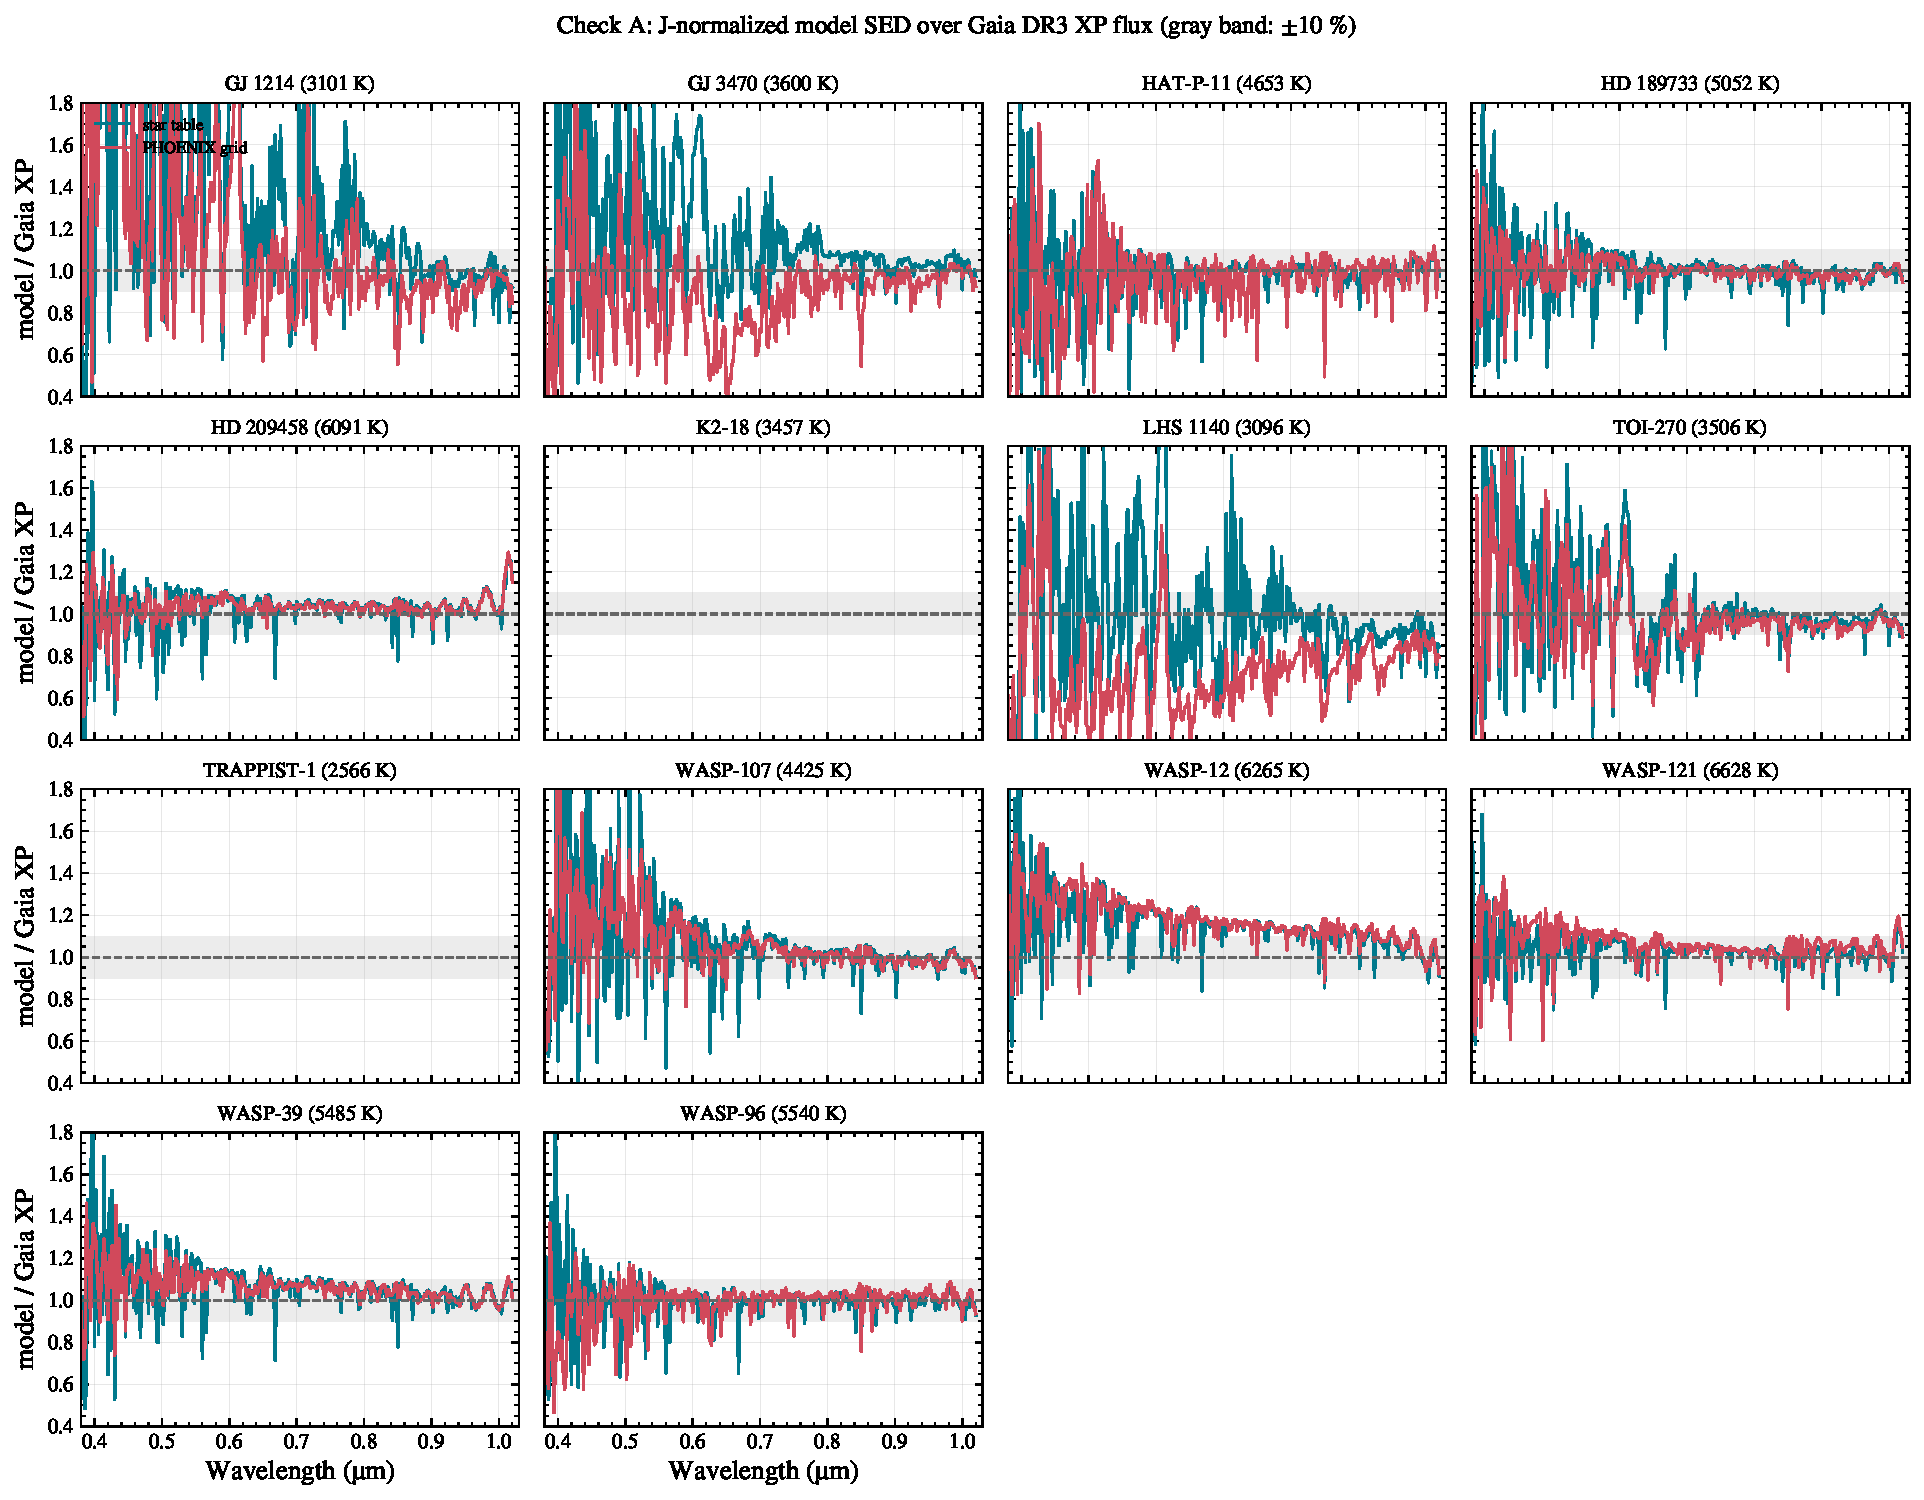
\includegraphics[width=\textwidth]{figures/checkA_sed_vs_xp.pdf}
\caption*{\footnotesize\textbf{Figure 1.} $J$-normalized model flux over the measured Gaia DR3 XP flux in 50\,nm bins, for the twelve hosts with an XP spectrum. Panels are ordered by $T_{\rm eff}$, coolest first. Blue circles: the committed star table that fed the noise tables; red squares: the parametric path's PHOENIX mini-grid. The XP flux errors per bin are smaller than the symbols; the gray band is $\pm10$\,\%; values above 2 are printed. A ratio above 1 means Lazuli's blue channels are predicted too bright by that factor. The common uptick in the last bin (1.00--1.05\,$\mu$m) is the red edge of the XP spectra, not a model feature. Derived here.}
\end{figure}

For seven of the eight hosts hotter than 4400\,K both models sit within the $\pm10$\,\% band over 0.40--1.02\,$\mu$m (blue ratios 0.95--1.11); WASP-12 (6265\,K) is 1.20--1.23 in the blue in both models and outside the band from 0.40 to 0.70\,$\mu$m. The M dwarfs fail. The star table over-predicts GJ~1214's blue flux by 1.40$\times$ and GJ~3470's by 1.20$\times$, consistent with the $V{-}J$ colours being 0.3--0.5\,mag too blue for GJ~1214 and TRAPPIST-1 (PHOENIX runs hot in the optical for late-M dwarfs). The parametric path's mini-grid is worse in a different way: LHS~1140 is 0.63$\times$ and GJ~3470 0.78$\times$ XP in the blue. Evaluating the grid at its nodes shows the cause: at 3100\,K the $[{\rm Fe/H}]=-0.5$, $\log g=5.0$ node and the $[{\rm Fe/H}]=+0.3,+0.5$ nodes at $\log g\le4.5$ have synthetic $V{-}J$ of 5.9--6.7 against 4.4--4.7 for their neighbours. The low-resolution non-solar pysynphot PHOENIX folders carry placeholder-like columns that the all-zero test in \texttt{make\_phoenix\_grid.py} does not catch, and trilinear interpolation drags every cool, non-solar host toward them (GitHub \#16). The pilot's WASP-96 anomaly ($\Delta(V{-}J)=+0.34$) is a catalog $V$ problem: its XP ratio is 0.99.

\subsection*{B. Photon budget and achieved precision}

\begin{table}[H]
\centering\small
\begin{tabular}{@{}lrrrrrrr@{}}
\toprule
\textbf{Planet} & \textbf{$J_{\rm Vega}$} & \textbf{$J_{\rm AB}$} & \textbf{MACC} & \textbf{$t_{\rm int}$ (s)} & \textbf{slicersim / hand} & \textbf{16th--84th pct.} & \textbf{var / signal} \\
\midrule
GJ 1214 b & 9.75 & 10.65 & 2:8:0 & 22.6 & 1.000 & 1.000--1.000 & 0.73 \\
GJ 3470 b & 8.79 & 9.69 & 2:4:0 & 11.3 & 1.000 & 1.000--1.000 & 0.73 \\
HAT-P-11 b & 7.61 & 8.51 & 2:1:0 & 2.8 & 1.000 & 1.000--1.000 & 1.07 \\
HD 189733 b & 6.07 & 6.97 & 2:1:0 & 2.8 & 1.000 & 1.000--1.000 & 1.17 \\
HD 209458 b & 6.59 & 7.49 & 2:1:0 & 2.8 & 1.000 & 1.000--1.000 & 1.05 \\
K2-18 b & 9.76 & 10.66 & 2:8:0 & 22.6 & 1.000 & 1.000--1.000 & 0.70 \\
LHS 1140 b & 9.61 & 10.51 & 2:8:0 & 22.6 & 1.000 & 1.000--1.000 & 0.72 \\
TOI-270 d & 9.10 & 10.00 & 2:4:0 & 11.3 & 1.000 & 1.000--1.000 & 0.74 \\
TRAPPIST-1 e & 11.35 & 12.25 & 8:8:0 & 158.5 & 1.000 & 1.000--1.000 & 1.22 \\
WASP-107 b & 9.38 & 10.28 & 2:8:0 & 22.6 & 1.000 & 1.000--1.000 & 0.68 \\
WASP-12 b & 10.48 & 11.38 & 2:8:0 & 22.6 & 1.000 & 1.000--1.000 & 0.69 \\
WASP-121 b & 9.62 & 10.52 & 2:8:0 & 22.6 & 1.000 & 1.000--1.000 & 0.68 \\
WASP-39 b & 10.66 & 11.56 & 4:8:0 & 67.9 & 1.000 & 1.000--1.000 & 0.93 \\
WASP-96 b & 11.27 & 12.17 & 4:8:0 & 67.9 & 1.000 & 1.000--1.000 & 0.93 \\
\bottomrule
\end{tabular}
\caption*{\footnotesize\textbf{Table B1.} Check B(i). Extracted slicersim signal over the hand photon budget $F_\lambda\,\lambda/(hc)\,A\,\eta\,{\rm QE}\,\Delta\lambda\,t_{\rm int}$ (median over 0.40--1.70\,$\mu$m, with the 16--84\% range), where $F_\lambda$ is the star table normalized here to the catalog $J$ with sncosmo and $A=7.07$\,m$^2$, $\eta$ and QE are read from the \texttt{lazuli\_cbe} configuration. MACC $n{:}m{:}d$ is the readout pattern (groups : frames averaged per group : dropped frames). The last column is the Rauscher et al.\ (2007) up-the-ramp variance over the Poisson variance of the accumulated signal. Derived here.}
\end{table}


The hand budget and slicersim agree to three decimals for all 14 hosts and in all three wavelength thirds. This closes the pilot's finding: with the Vega-to-AB conversion in \texttt{slicer.depth\_error}, the magnitude system, collecting area, throughput, quantum efficiency, channel width and integration time are all applied once and consistently. The variance-over-signal column is the Rauscher et al.\ (2007) up-the-ramp expression: below 1 for the frame-averaged (2,8,0) and (2,4,0) ramps, above 1 where read noise contributes ((2,1,0) ramps on the bright hosts; (8,8,0) on TRAPPIST-1).

\begin{table}[H]
\centering\scriptsize
\begin{tabular}{@{}lllrrrrrr@{}}
\toprule
\textbf{Planet} & \textbf{Dataset} & \textbf{Fac.} & \textbf{$n$} & \textbf{bin ($\mu$m)} & \textbf{achieved $\sigma$} & \textbf{Lazuli $\sigma_1$} & \textbf{ratio} & \textbf{area-only} \\
\midrule
GJ 1214 b & Berta et al. 2012 & HST & 24 & 0.023 & 212 & 77 & 0.36$\downarrow$ & 0.75 \\
GJ 1214 b & Kreidberg et al. 2014 & HST & 22 & 0.023 & 28 & 76 & 2.74 & 0.75 \\
GJ 3470 b & Benneke et al. 2019 & HST & 8 & 0.049 & 101 & 37 & 0.35$\downarrow$ & 0.75 \\
GJ 3470 b & Benneke et al. 2019 & HST & 18 & 0.030 & 32 & 28 & 0.92 & 0.75 \\
GJ 3470 b & Ehrenreich et al. 2014 & HST & 107 & 0.005 & 398 & 73 & 0.18$\downarrow$ & 0.75 \\
HAT-P-11 b & Fraine et al. 2014 & HST & 29 & 0.019 & 43 & 24 & 0.59$\downarrow$ & 0.75 \\
HD 189733 b & McCullough et al. 2014 & HST & 28 & 0.019 & 120 & 19 & 0.15$\downarrow$ & 0.75 \\
HD 189733 b & Pont et al. 2013 & HST & 10 & 0.025 & 39 & 16 & 0.40$\downarrow$ & 0.75 \\
HD 189733 b & Pont et al. 2013 & HST & 6 & 0.027 & 246 & 14 & 0.07$\downarrow$ & 0.75 \\
HD 189733 b & Pont et al. 2013 & HST & 12 & 0.017 & 70 & 19 & 0.32$\downarrow$ & 0.75 \\
HD 189733 b & Sing et al. 2016 & HST & 18 & 0.025 & 41 & 16 & 0.38$\downarrow$ & 0.75 \\
HD 189733 b & Sing et al. 2016 & HST & 29 & 0.009 & 68 & 23 & 0.31$\downarrow$ & 0.75 \\
HD 209458 b & Deming et al. 2013 & HST & 28 & 0.019 & 35 & 15 & 0.40$\downarrow$ & 0.75 \\
HD 209458 b & Sing et al. 2016 & HST & 81 & 0.004 & 85 & 28 & 0.35$\downarrow$ & 0.75 \\
HD 209458 b & Sing et al. 2016 & HST & 29 & 0.009 & 34 & 21 & 0.60$\downarrow$ & 0.75 \\
K2-18 b & Benneke et al. 2019 & HST & 17 & 0.030 & 23 & 37 & 1.63 & 0.75 \\
K2-18 b & Tsiaras et al. 2019 & HST & 17 & 0.028 & 24 & 39 & 1.63 & 0.75 \\
WASP-107 b & Kreidberg et al. 2018 & HST & 20 & 0.026 & 57 & 34 & 0.59$\downarrow$ & 0.75 \\
WASP-107 b & Spake et al. 2018 & HST & 49 & 0.024 & 69 & 35 & 0.66$\downarrow$ & 0.75 \\
WASP-12 b & Kreidberg et al. 2015 & HST & 13 & 0.069 & 51 & 32 & 0.65$\downarrow$ & 0.75 \\
WASP-12 b & Mandell et al. 2013 & HST & 19 & 0.027 & 229 & 56 & 0.24$\downarrow$ & 0.75 \\
WASP-12 b & Sing et al. 2013 & HST & 20 & 0.052 & 125 & 37 & 0.29$\downarrow$ & 0.75 \\
WASP-12 b & Stevenson et al. 2014 & HST & 29 & 0.015 & 100 & 58 & 0.47$\downarrow$ & 0.75 \\
WASP-121 b & Evans et al. 2016 & HST & 31 & 0.019 & 87 & 45 & 0.50$\downarrow$ & 0.75 \\
WASP-39 b & Feinstein et al. 2022 & JWST & 213 & 0.004 & 60 & 136 & 2.30 & 1.90 \\
WASP-39 b & Fischer et al. 2016 & HST & 31 & 0.010 & 263 & 99 & 0.36$\downarrow$ & 0.75 \\
WASP-39 b & Rustamkulov et al. 2022 & JWST & 63 & 0.006 & 85 & 117 & 1.17$\downarrow$ & 1.90 \\
WASP-39 b & Sing et al. 2016 & HST & 31 & 0.010 & 281 & 104 & 0.36$\downarrow$ & 0.75 \\
WASP-39 b & Wakeford et al. 2018 & HST & 36 & 0.019 & 172 & 66 & 0.41$\downarrow$ & 0.75 \\
\bottomrule
\end{tabular}
\caption*{\footnotesize\textbf{Table B2.} Check B(ii). Published per-bin depth precision inside 0.40--1.70\,$\mu$m (median, ppm, as tabulated in the NASA Exoplanet Archive) against lazuli-exo's predicted single-transit precision for the same bins (committed noise tables; statistical noise only). ``area-only'' is $\sqrt{A_{\rm other}/A_{\rm Lazuli}}$ with $A_{\rm HST}=4.0$, $A_{\rm JWST}=25.4$, $A_{\rm Lazuli}=7.07$\,m$^2$; $\downarrow$ marks datasets where Lazuli's predicted error is smaller than that scaling. The archive does not record the number of visits combined, so ratios are indicative. Derived here.}
\end{table}


\begin{figure}[H]
\centering
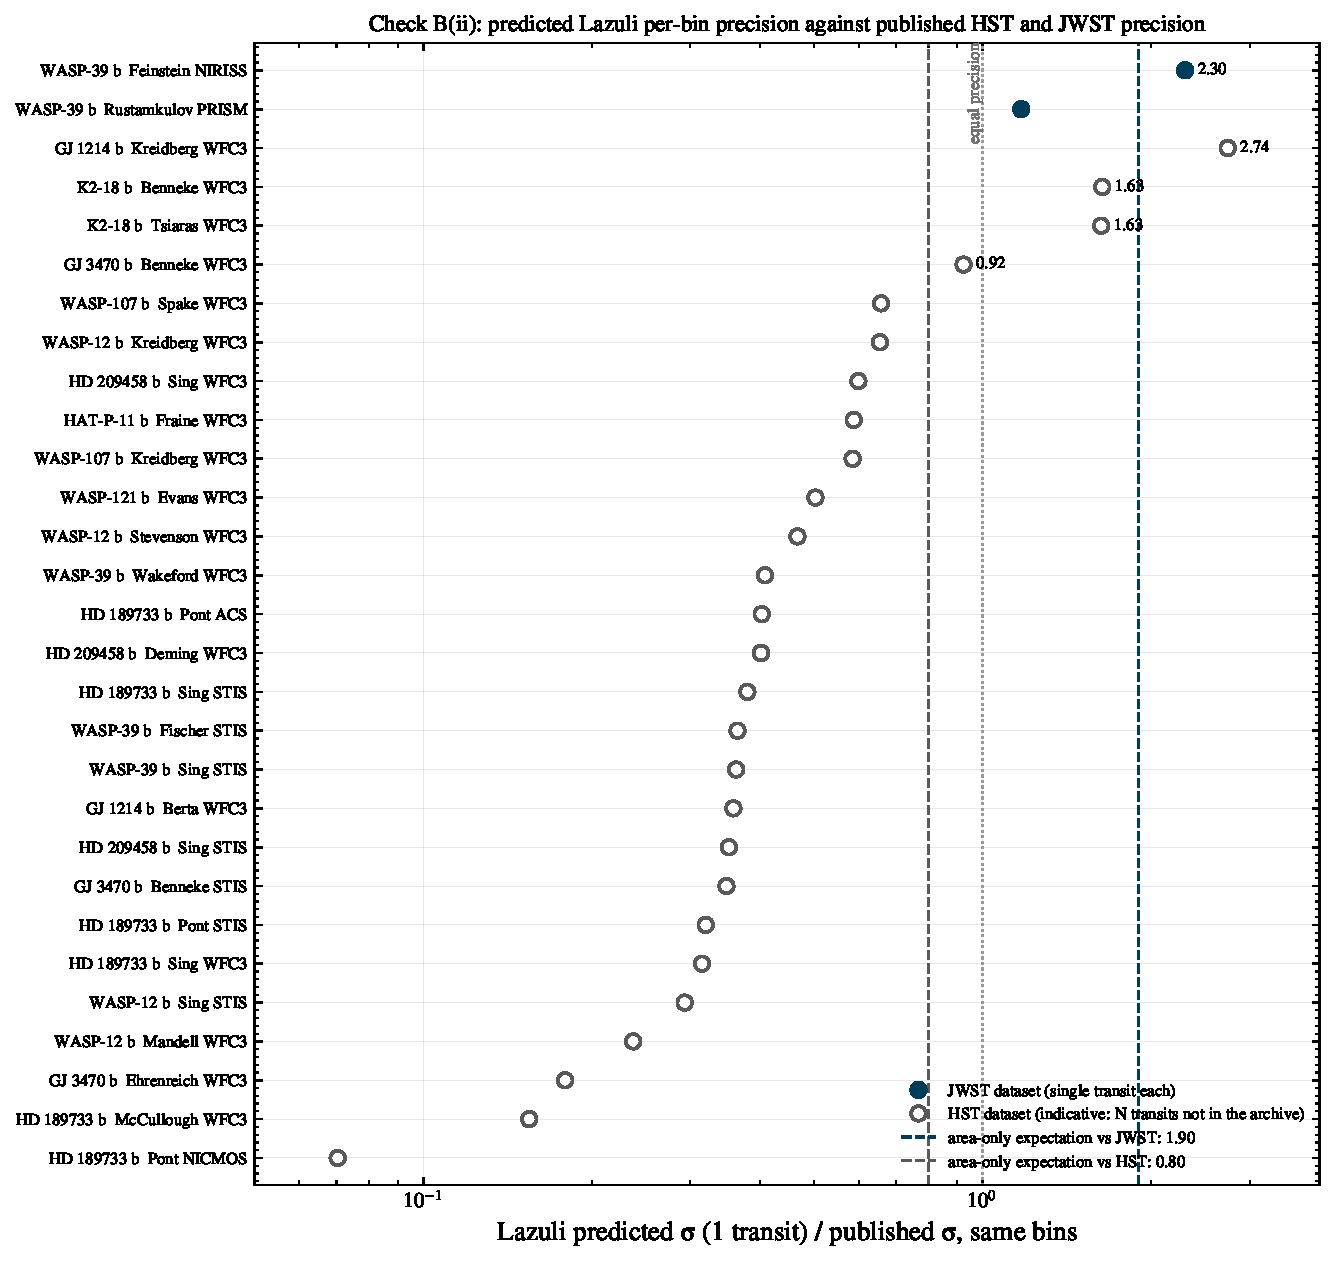
\includegraphics[width=\textwidth]{figures/checkB_precision_ratio.pdf}
\caption*{\footnotesize\textbf{Figure 2.} Lazuli's predicted single-transit per-bin precision divided by the published per-bin precision of each dataset in Table~B2, same bins; JWST datasets (filled, single transit each) at the top, HST datasets (hollow; number of transits not recorded in the archive) sorted by ratio. Dashed lines: the ratio expected from collecting area alone, $\sqrt{A_{\rm other}/A_{\rm Lazuli}}$ (1.90 vs JWST, 0.80 vs HST). A point to the right of its dashed line means Lazuli is predicted to do worse than area scaling against that dataset. A point to the left can mean that the published dataset did not reach its photon limit, that it combined several transits, or that Lazuli's statistical-only error is too small; the memo cannot separate these for HST. Derived here.}
\end{figure}

The two JWST datasets are the clean comparison (Figure~2). For WASP-39\,b, lazuli-exo predicts a single-transit precision of 136\,ppm in the 0.004\,$\mu$m NIRISS/SOSS bins where Feinstein et al.\ (2023) achieved 60\,ppm, a ratio of 2.3 against 1.9 from collecting area alone; against the PRISM bins of Rustamkulov et al.\ (2023) the ratio is 1.2 (Figure~2). Given that NIRISS and PRISM throughputs and their partial-saturation handling for a $J=10.7$ star are not in this comparison, the predicted Lazuli precision is consistent with photon-limited scaling to within a factor 1.5. Against HST, Lazuli predicts errors 0.07--0.66$\times$ the published per-bin values for 23 of 27 datasets, far below the 0.80 area ratio. HST's $\sim$50\,\% orbital duty cycle, scanning overheads and systematics explain much of that, but a statistical-only Lazuli bar that is too small cannot be excluded from this comparison, so lazuli-exo's bars are a floor, not a forecast. The exceptions (K2-18\,b at 1.6 in both reductions, GJ~1214\,b Kreidberg et al.\ at 2.7, GJ~3470\,b Benneke et al.\ WFC3 at 0.9) are multi-transit programs compared here with one Lazuli transit; the archive does not record their transit counts, and checking each against its paper (ratio $\approx 0.80\sqrt{N}$ if photon-limited) is an action item. HD~189733\,b and HD~209458\,b sit on saturated noise tables and are flagged unvalidated in the code.

\subsection*{C. White-light geometry}

\begin{table}[H]
\centering\footnotesize
\begin{tabular}{@{}lrrrrrlrrr@{}}
\toprule
\textbf{Planet} & \textbf{$t_{14}^{\rm geo}/t_{14}$} & \textbf{$b$} & \textbf{$n_{\rm ref}$} & \textbf{$\Delta k/k$} & \textbf{$\Delta\delta$ (ppm)} & \textbf{latest reference} & \textbf{$k/k_{\rm reg}$} & \textbf{$a/R_\star$ ratio} & \textbf{$t_{14}^{\rm geo}/t_{14}^{\rm reg}$} \\
\midrule
GJ 1214 b & 1.000 & 0.26 & 8 & 0.031 & 850 & Mahajan et al. 2024 & 1.000 & 1.000 & 1.000 \\
GJ 3470 b & 1.014 & 0.21 & 4 & 0.044 & 525 & Kokori et al. 2023 & 1.000 & 0.994 & 1.008 \\
HAT-P-11 b & 0.847 & 0.24 & 10 & 0.024 & 162 & Basilicata et al. 2024 & 1.017 & 0.900 & 1.107 \\
HD 189733 b & 1.001 & 0.66 & 6 & 0.040 & 1925 & Kokori et al. 2023 & 1.000 & 1.009 & 0.995 \\
HD 209458 b & 0.999 & 0.51 & 3 & 0.001 & 34 & Kokori et al. 2023 & 1.000 & 0.994 & 1.006 \\
K2-18 b & 0.966 & 0.60 & 0 & -- & -- & -- & -- & -- & -- \\
LHS 1140 b & 0.928 & 0.22 & 4 & 0.042 & 449 & Kokori et al. 2023 & 1.000 & 1.000 & 0.976 \\
TOI-270 d & 1.007 & 0.23 & 3 & 0.027 & 141 & Mikal-Evans et al. 202 & 1.075 & 1.001 & 1.009 \\
TRAPPIST-1 e & 0.995 & 0.19 & 1 & 0.000 & 0 & Agol et al. 2021 & 1.000 & 1.000 & 1.000 \\
WASP-107 b & 1.008 & 0.12 & 4 & 0.011 & 464 & Wu et al. 2026 & 1.000 & 1.000 & 1.008 \\
WASP-12 b & 1.023 & 0.45 & 4 & 0.017 & 472 & Kokori et al. 2023 & 1.007 & 1.013 & 0.998 \\
WASP-121 b & 0.997 & 0.10 & 4 & 0.028 & 847 & Kokori et al. 2023 & 1.016 & 0.992 & 1.010 \\
WASP-39 b & 0.987 & 0.53 & 3 & 0.023 & 951 & Kokori et al. 2023 & 1.000 & 0.998 & 1.028 \\
WASP-96 b & 1.014 & 0.71 & 2 & 0.020 & 560 & Kokori et al. 2023 & 0.980 & 1.000 & 1.010 \\
\bottomrule
\end{tabular}
\caption*{\footnotesize\textbf{Table C1.} Check C, part 1. Column 2: $t_{14}$ recomputed from the registry's own $(a/R_\star, i, e, \omega, k)$ over the registry $t_{14}$. Columns 4--6: number of archive solutions with $(k, a/R_\star, i)$, their spread in $k$ and in white-light depth. Columns 7--10: the most recent such solution against the registry. Derived here.}
\end{table}
\begin{table}[H]
\centering\small
\begin{tabular}{@{}lrrrrrr@{}}
\toprule
\textbf{Planet} & \textbf{solver (ppm)} & \textbf{local arc (ppm)} & \textbf{$\sigma_{\rm pt}$ (ppm)} & \textbf{$t_{14}^{\rm batman}/t_{14}^{\rm reg}$} & \textbf{LD $I<0$} & \textbf{max $u_1{+}u_2$} \\
\midrule
GJ 1214 b & 0.01 & 0.7 & 72 & 0.998 & 0 & 0.938 \\
GJ 3470 b & 0.01 & 2.2 & 63 & 1.014 & 0 & 0.888 \\
HAT-P-11 b & 0.01 & 23.7 & 43 & 0.844 & 0 & 0.887 \\
HD 189733 b & 0.01 & 0.0 & 32 & 0.999 & 0 & 0.914 \\
HD 209458 b & 0.01 & 0.0 & 25 & 0.999 & 0 & 0.874 \\
K2-18 b & 0.01 & 18.6 & 70 & 0.961 & 0 & 0.899 \\
LHS 1140 b & 0.01 & 0.0 & 68 & 0.924 & 0 & 0.949 \\
TOI-270 d & 0.01 & 0.2 & 74 & 1.004 & 0 & 0.857 \\
TRAPPIST-1 e & 0.01 & 0.0 & 77 & 0.920 & 6 & 1.048 \\
WASP-107 b & 0.07 & 5.8 & 54 & 1.001 & 0 & 0.895 \\
WASP-12 b & 0.01 & 68.8 & 79 & 1.014 & 0 & 0.864 \\
WASP-121 b & 0.07 & 7.2 & 52 & 0.996 & 0 & 0.857 \\
WASP-39 b & 0.01 & 0.0 & 61 & 0.978 & 0 & 0.903 \\
WASP-96 b & 0.01 & 0.0 & 81 & 1.006 & 0 & 0.897 \\
\bottomrule
\end{tabular}
\caption*{\footnotesize\textbf{Table C2.} Check C, part 2. Numpy transit solver vs batman at identical separations (max $|\Delta F|$); lazuli-exo's local-arc $z(t)$ vs batman's Keplerian $z(t)$ for the white-light curve; the per-sample noise at native cadence for one transit; batman's $t_{14}$ from the registry geometry over the registry $t_{14}$; number of LD chunks with negative limb intensity. Derived here.}
\end{table}


The registry's own $(a/R_\star, i, e, \omega, k)$ reproduce its $t_{14}$ within 3.5\,\% for twelve targets but give 0.85$\times$ for HAT-P-11\,b and 0.93$\times$ for LHS~1140\,b, confirming the audit's finding with independent per-reference solutions. Published $k$ values spread by 1--4\,\% for the eleven targets with two or more solutions, which is 140--1900\,ppm in white-light depth (HD~209458\,b, with three nearly identical solutions, 34\,ppm), against a Lazuli single-transit white-light depth error of 2--25\,ppm (Table~C2, $\sigma_\delta$). The numpy solver agrees with batman to 0.07\,ppm; the local circular-arc $z(t)$ is within 1\,ppm for circular orbits and off by 19--69\,ppm for the eccentric or grazing ones, i.e.\ 0.27, 0.56 and 0.87 of the per-sample noise for K2-18\,b, HAT-P-11\,b and WASP-12\,b, all above the 0.2$\sigma_{\rm pt}$ criterion of Table~3. TRAPPIST-1\,e's limb-darkening table has six chunks with negative limb intensity at 0.41--0.74\,$\mu$m, overlapping the 0.6--1.0\,$\mu$m band used in check G; the light curves, not the depth tables, are affected (GitHub \#10).

\subsection*{D. Spectral shape}

\begin{table}[H]
\centering\scriptsize
\begin{tabular}{@{}lllrrrlrrrrrrl@{}}
\toprule
\textbf{Planet} & \textbf{Dataset} & \textbf{Fac.} & \textbf{$n$} & \textbf{amp} & \textbf{$\sigma$} & \textbf{best} & \textbf{$\chi^2_\nu$} & \textbf{$\chi^2_{\nu,\rm flat}$} & \textbf{$b_{\rm clear}$} & \textbf{$b_{\rm cloudy}$} & \textbf{$b_{\rm hazy}$} & \textbf{$b_{\rm high\text{-}met}$} & \textbf{brk.} \\
\midrule
GJ 1214 b & Bean et al. 2011, MMIRS & grou & 36 & 1032 & 175 & flat & 1.3 & 1.3 & -0.09 & 0.30 & 0.41 & -0.18 & no \\
GJ 1214 b & Berta et al. 2012, WFC3 & HST & 24 & 778 & 212 & cloudy & 0.6 & 0.8 & 0.17 & 1.24 & 0.18 & 0.19 & yes \\
GJ 1214 b & Croll et al. 2011, WIRCam & grou & 5 & 780 & 340 & cloudy & 0.9 & 0.9 & 0.26 & 1.49 & 0.28 & 0.50 & yes \\
GJ 1214 b & Kreidberg et al. 2014, Wide Field C & HST & 22 & 99 & 28 & flat & 1.0 & 1.0 & 0.01 & 0.09 & 0.01 & 0.01 & no \\
GJ 1214 b & Rackham et al. 2017, IMACS spectr & grou & 14 & 619 & 185 & flat & 0.8 & 0.8 & -0.16 & -3.48 & -0.41 & 0.16 & no \\
GJ 1214 b & Wilson et al. 2014, OSIRIS & grou & 8 & 2299 & 423 & hazy & 4.0 & 4.4 & 0.55 & 53.00 & 5.20 & -0.33 & yes \\
GJ 3470 b & Benneke et al. 2019, Space Telesc & HST & 8 & 303 & 101 & cloudy & 1.2 & 1.2 & 0.13 & 0.96 & -0.21 & 0.25 & no \\
GJ 3470 b & Benneke et al. 2019, Wide Field C & HST & 18 & 161 & 32 & cloudy & 2.3 & 2.3 & 0.08 & 0.50 & 0.09 & 0.11 & no \\
GJ 3470 b & Biddle et al. 2014,  & grou & 8 & 1536 & 291 & hazy & 0.9 & 1.3 & 0.40 & -95.75 & 2.28 & -1.77 & yes \\
GJ 3470 b & Biddle et al. 2014, SBIG imager & grou & 5 & 596 & 402 & hazy & 0.3 & 0.8 & 3.81 & -45.23 & 2.27 & -1.76 & yes \\
GJ 3470 b & Dragomir et al. 2015, SBIG imager & grou & 7 & 1492 & 476 & hazy & 0.5 & 0.9 & -0.74 & 99.69 & 2.65 & 7.62 & yes \\
GJ 3470 b & Ehrenreich et al. 2014, Wide Field C & HST & 107 & 2598 & 398 & cloudy & 1.4 & 1.4 & 0.20 & 0.81 & 0.20 & 0.38 & no \\
HAT-P-11 b & Fraine et al. 2014, Wide Field C & HST & 29 & 247 & 43 & high-met & 1.0 & 2.0 & 0.50 & 3.24 & 0.53 & 0.81 & yes \\
HD 189733 b & Barnes et al. 2016, HARPS Echell & grou & 5 & 4500 & 1100 & clear & 2.6 & 2.6 & -- & -- & -- & -- & no \\
HD 189733 b & Borsa et al. 2016, HARPS Echell & grou & 7 & 676 & 149 & hazy & 0.5 & 1.9 & -0.86 & 0.51 & 2.10 & -1.03 & yes \\
HD 189733 b & Di Gloria et al. 2015, HARPS Echell & grou & 6 & 1152 & 365 & hazy & 0.9 & 1.1 & -2.43 & -11.40 & 2.68 & -2.30 & yes \\
HD 189733 b & McCullough et al. 2014, Wide Field C & HST & 28 & 352 & 120 & high-met & 0.4 & 0.6 & 0.44 & 2.50 & 0.46 & 0.65 & yes \\
HD 189733 b & Pont et al. 2013, Advanced Cam & HST & 10 & 461 & 39 & hazy & 1.2 & 6.5 & 0.63 & 4.73 & 0.78 & 0.85 & yes \\
HD 189733 b & Pont et al. 2013, Near Infrare & HST & 6 & 1051 & 246 & flat & 2.8 & 2.8 & -2.15 & -15.42 & -2.17 & -3.13 & no \\
HD 189733 b & Pont et al. 2013, Space Telesc & HST & 12 & 401 & 70 & hazy & 2.7 & 4.5 & 0.03 & 0.48 & 0.67 & -0.03 & no \\
HD 189733 b & Sing et al. 2016, Space Telesc & HST & 18 & 643 & 41 & hazy & 2.3 & 18.8 & 0.48 & 1.48 & 0.95 & 0.31 & yes \\
HD 189733 b & Sing et al. 2016, Wide Field C & HST & 29 & 353 & 68 & high-met & 1.1 & 1.9 & 0.43 & 2.46 & 0.46 & 0.64 & yes \\
HD 209458 b & Deming et al. 2013, Wide Field C & HST & 28 & 276 & 35 & cloudy & 1.6 & 5.9 & 0.32 & 1.07 & 0.33 & 0.52 & yes \\
HD 209458 b & Sing et al. 2016, Space Telesc & HST & 81 & 701 & 85 & cloudy & 1.9 & 2.0 & 0.32 & 1.58 & 0.17 & 0.17 & yes \\
HD 209458 b & Sing et al. 2016, Wide Field C & HST & 29 & 262 & 34 & cloudy & 2.6 & 5.1 & 0.26 & 0.79 & 0.27 & 0.43 & no \\
K2-18 b & Benneke et al. 2019, Wide Field C & HST & 17 & 102 & 23 & high-met & 1.2 & 1.9 & 0.60 & 5.16 & 0.63 & 0.91 & yes \\
K2-18 b & Tsiaras et al. 2019, Wide Field C & HST & 17 & 115 & 24 & high-met & 1.2 & 1.6 & 0.44 & 4.32 & 0.45 & 0.78 & yes \\
WASP-107 b & Kreidberg et al. 2018, Wide Field C & HST & 20 & 433 & 57 & flat & 6.5 & 6.5 & 0.09 & 0.39 & 0.10 & 0.18 & no \\
WASP-107 b & Spake et al. 2018, Wide Field C & HST & 49 & 623 & 69 & flat & 6.1 & 6.1 & 0.07 & 0.41 & 0.09 & 0.14 & no \\
WASP-12 b & Kreidberg et al. 2015, Wide Field C & HST & 13 & 273 & 51 & cloudy & 2.8 & 4.0 & 0.23 & 4.02 & 0.30 & 0.45 & yes \\
WASP-12 b & Mandell et al. 2013, Wide Field C & HST & 19 & 646 & 229 & high-met & 0.4 & 0.6 & 0.69 & 5.21 & 0.70 & 1.43 & yes \\
WASP-12 b & Sing et al. 2013, Space Telesc & HST & 20 & 569 & 125 & flat & 1.8 & 1.8 & -0.34 & -3.56 & 0.22 & -0.36 & no \\
WASP-12 b & Stevenson et al. 2014, Wide Field C & HST & 29 & 1170 & 100 & flat & 7.6 & 7.6 & -0.59 & -9.11 & -0.82 & -1.14 & no \\
WASP-121 b & Evans et al. 2016, Wide Field C & HST & 31 & 1388 & 87 & cloudy & 4.0 & 4.2 & 0.08 & 0.75 & 0.32 & -0.19 & no \\
WASP-39 b & Feinstein et al. 2022, Near Infrare & JWST & 213 & 982 & 60 & cloudy & 5.4 & 13.1 & 0.22 & 0.82 & 0.23 & 0.33 & no \\
WASP-39 b & Fischer et al. 2016, Space Telesc & HST & 31 & 2067 & 263 & cloudy & 1.0 & 1.1 & 0.30 & 1.20 & 0.11 & 0.08 & yes \\
WASP-39 b & Nikolov et al. 2016, FORS2 & grou & 28 & 2017 & 327 & cloudy & 0.7 & 1.2 & 0.38 & 0.84 & 0.19 & 0.33 & no \\
WASP-39 b & Rustamkulov et al. 202, Near Infrare & JWST & 63 & 1337 & 85 & cloudy & 6.2 & 8.3 & 0.29 & 0.69 & 0.24 & 0.37 & no \\
WASP-39 b & Sing et al. 2016, Space Telesc & HST & 31 & 2122 & 281 & cloudy & 1.8 & 1.9 & 0.27 & 1.69 & 0.32 & -0.13 & yes \\
WASP-39 b & Wakeford et al. 2018, Wide Field C & HST & 36 & 1128 & 172 & cloudy & 2.7 & 6.0 & 0.33 & 1.22 & 0.40 & 0.45 & yes \\
WASP-96 b & Nikolov et al. 2018, FORS2 & grou & 48 & 1135 & 221 & clear & 1.0 & 1.5 & 0.78 & 1.82 & 0.29 & 0.80 & yes \\
TRAPPIST-1 e & Espinoza et al. 2025, , HST\_WFC3IR\_v & HST & 12 & 600 & 150 & flat & 1.4 & 1.4 & -0.07 & -0.00 & -0.08 & -0.22 & no \\
TRAPPIST-1 e & Espinoza et al. 2025, , HST\_WFC3IR\_v & HST & 12 & 690 & 130 & flat & 2.2 & 2.2 & -0.24 & -1.65 & -0.24 & -0.23 & no \\
TRAPPIST-1 e & Espinoza et al. 2025, , JWST\_PRISM\_E & JWST & 32 & 2045 & 152 & flat & 1.2 & 1.2 & 0.02 & -0.09 & 0.00 & 0.05 & no \\
TRAPPIST-1 e & Espinoza et al. 2025, , JWST\_PRISM\_E & JWST & 32 & 6099 & 167 & flat & 0.7 & 0.7 & 0.08 & 0.46 & 0.07 & 0.08 & no \\
TRAPPIST-1 e & Espinoza et al. 2025, , JWST\_PRISM\_E & JWST & 32 & 2115 & 129 & flat & 1.0 & 1.0 & 0.01 & -0.01 & 0.04 & 0.02 & no \\
TRAPPIST-1 e & Espinoza et al. 2025, , JWST\_PRISM\_E & JWST & 32 & 3343 & 214 & flat & 0.8 & 0.8 & -0.02 & -0.18 & -0.06 & -0.04 & no \\
\bottomrule
\end{tabular}
\caption*{\footnotesize\textbf{Table D1.} Committed POSEIDON tables. Check D. Every dataset with $\ge 5$ points and errors inside 0.40--1.70\,$\mu$m (NASA Exoplanet Archive; TRAPPIST-1\,e from Espinoza et al.\ 2025). ``amp'' and $\sigma$: measured peak-to-peak depth and median error (ppm). ``best'' is the scenario with the lowest offset-fit $\chi^2_\nu$ (also given for the flat scenario); $b$ is the fitted data/model amplitude ratio (1 = the scenario has the measured amplitude); ``brk.'' = the four atmospheric scenarios' $b$ values straddle 1. Derived here.}
\end{table}
\begin{table}[H]
\centering\scriptsize
\begin{tabular}{@{}lllrrrlrrrrrrl@{}}
\toprule
\textbf{Planet} & \textbf{Dataset} & \textbf{Fac.} & \textbf{$n$} & \textbf{amp} & \textbf{$\sigma$} & \textbf{best} & \textbf{$\chi^2_\nu$} & \textbf{$\chi^2_{\nu,\rm flat}$} & \textbf{$b_{\rm clear}$} & \textbf{$b_{\rm cloudy}$} & \textbf{$b_{\rm hazy}$} & \textbf{$b_{\rm high\text{-}met}$} & \textbf{brk.} \\
\midrule
GJ 1214 b & Bean et al. 2011, MMIRS & grou & 36 & 1032 & 175 & flat & 1.3 & 1.3 & -0.07 & -0.00 & 0.44 & -0.21 & no \\
GJ 1214 b & Berta et al. 2012, WFC3 & HST & 24 & 778 & 212 & cloudy & 0.6 & 0.8 & 0.22 & 2.32 & 0.24 & 0.24 & yes \\
GJ 1214 b & Croll et al. 2011, WIRCam & grou & 5 & 780 & 340 & high-met & 0.8 & 0.9 & 0.33 & 2.66 & 0.36 & 0.62 & yes \\
GJ 1214 b & Kreidberg et al. 2014, Wide Field C & HST & 22 & 99 & 28 & flat & 1.0 & 1.0 & 0.02 & 0.16 & 0.02 & 0.02 & no \\
GJ 1214 b & Rackham et al. 2017, IMACS spectr & grou & 14 & 619 & 185 & flat & 0.8 & 0.8 & -0.23 & -7.57 & -0.53 & 0.18 & no \\
GJ 1214 b & Wilson et al. 2014, OSIRIS & grou & 8 & 2299 & 423 & clear & 4.0 & 4.4 & 1.20 & 119.41 & 4.72 & -0.39 & yes \\
GJ 3470 b & Benneke et al. 2019, Space Telesc & HST & 8 & 303 & 101 & cloudy & 1.2 & 1.2 & 0.17 & 1.86 & -0.20 & 0.31 & yes \\
GJ 3470 b & Benneke et al. 2019, Wide Field C & HST & 18 & 161 & 32 & cloudy & 1.6 & 2.3 & 0.11 & 0.95 & 0.12 & 0.13 & no \\
GJ 3470 b & Biddle et al. 2014,  & grou & 8 & 1536 & 291 & hazy & 1.0 & 1.3 & 3.81 & -140.76 & 3.30 & -2.20 & yes \\
GJ 3470 b & Biddle et al. 2014, SBIG imager & grou & 5 & 596 & 402 & hazy & 0.4 & 0.8 & 4.19 & -38.78 & 3.11 & -2.15 & yes \\
GJ 3470 b & Dragomir et al. 2015, SBIG imager & grou & 7 & 1492 & 476 & hazy & 0.7 & 0.9 & -1.16 & 229.20 & 4.23 & 13.27 & yes \\
GJ 3470 b & Ehrenreich et al. 2014, Wide Field C & HST & 107 & 2598 & 398 & cloudy & 1.4 & 1.4 & 0.26 & 1.40 & 0.27 & 0.48 & yes \\
HAT-P-11 b & Fraine et al. 2014, Wide Field C & HST & 29 & 247 & 43 & high-met & 0.9 & 2.0 & 0.58 & 5.18 & 0.62 & 0.93 & yes \\
HD 189733 b & Barnes et al. 2016, HARPS Echell & grou & 5 & 4500 & 1100 & clear & 2.6 & 2.6 & -- & -- & -- & -- & no \\
HD 189733 b & Borsa et al. 2016, HARPS Echell & grou & 7 & 676 & 149 & hazy & 0.8 & 1.9 & -0.90 & 1.32 & 2.63 & -1.08 & yes \\
HD 189733 b & Di Gloria et al. 2015, HARPS Echell & grou & 6 & 1152 & 365 & hazy & 0.9 & 1.1 & -2.56 & -13.45 & 3.03 & -2.41 & yes \\
HD 189733 b & McCullough et al. 2014, Wide Field C & HST & 28 & 352 & 120 & high-met & 0.3 & 0.6 & 0.46 & 3.12 & 0.48 & 0.68 & yes \\
HD 189733 b & Pont et al. 2013, Advanced Cam & HST & 10 & 461 & 39 & hazy & 1.3 & 6.5 & 0.66 & 6.07 & 0.79 & 0.88 & yes \\
HD 189733 b & Pont et al. 2013, Near Infrare & HST & 6 & 1051 & 246 & flat & 2.8 & 2.8 & -2.26 & -20.39 & -2.29 & -3.27 & no \\
HD 189733 b & Pont et al. 2013, Space Telesc & HST & 12 & 401 & 70 & hazy & 4.0 & 4.5 & 0.03 & 0.59 & 0.54 & -0.03 & no \\
HD 189733 b & Sing et al. 2016, Space Telesc & HST & 18 & 643 & 41 & hazy & 3.6 & 18.8 & 0.50 & 1.79 & 0.97 & 0.33 & yes \\
HD 189733 b & Sing et al. 2016, Wide Field C & HST & 29 & 353 & 68 & high-met & 1.1 & 1.9 & 0.46 & 3.07 & 0.48 & 0.67 & yes \\
HD 209458 b & Deming et al. 2013, Wide Field C & HST & 28 & 276 & 35 & cloudy & 2.1 & 5.9 & 0.35 & 1.48 & 0.37 & 0.58 & yes \\
HD 209458 b & Sing et al. 2016, Space Telesc & HST & 81 & 701 & 85 & cloudy & 1.9 & 2.0 & 0.36 & 2.32 & 0.25 & 0.19 & yes \\
HD 209458 b & Sing et al. 2016, Wide Field C & HST & 29 & 262 & 34 & cloudy & 2.5 & 5.1 & 0.29 & 1.07 & 0.30 & 0.47 & yes \\
K2-18 b & Benneke et al. 2019, Wide Field C & HST & 17 & 102 & 23 & high-met & 1.2 & 1.9 & 0.69 & 7.91 & 0.73 & 1.05 & yes \\
K2-18 b & Tsiaras et al. 2019, Wide Field C & HST & 17 & 115 & 24 & high-met & 1.1 & 1.6 & 0.50 & 6.73 & 0.53 & 0.89 & yes \\
WASP-107 b & Kreidberg et al. 2018, Wide Field C & HST & 20 & 433 & 57 & cloudy & 2.0 & 6.5 & 0.12 & 0.76 & 0.14 & 0.25 & no \\
WASP-107 b & Spake et al. 2018, Wide Field C & HST & 49 & 623 & 69 & cloudy & 3.5 & 6.1 & 0.09 & 0.80 & 0.12 & 0.19 & no \\
WASP-12 b & Kreidberg et al. 2015, Wide Field C & HST & 13 & 273 & 51 & cloudy & 3.2 & 4.0 & 0.26 & 6.10 & 0.33 & 0.56 & yes \\
WASP-12 b & Mandell et al. 2013, Wide Field C & HST & 19 & 646 & 229 & hazy & 0.4 & 0.6 & 0.79 & 8.96 & 0.82 & 1.84 & yes \\
WASP-12 b & Sing et al. 2013, Space Telesc & HST & 20 & 569 & 125 & flat & 1.8 & 1.8 & -0.39 & -6.52 & 0.22 & -0.42 & no \\
WASP-12 b & Stevenson et al. 2014, Wide Field C & HST & 29 & 1170 & 100 & flat & 7.6 & 7.6 & -0.67 & -14.39 & -0.88 & -1.39 & no \\
WASP-121 b & Evans et al. 2016, Wide Field C & HST & 31 & 1388 & 87 & cloudy & 4.0 & 4.2 & 0.10 & 1.22 & 0.35 & -0.25 & yes \\
WASP-39 b & Feinstein et al. 2022, Near Infrare & JWST & 213 & 982 & 60 & cloudy & 5.9 & 13.1 & 0.28 & 1.38 & 0.30 & 0.41 & yes \\
WASP-39 b & Fischer et al. 2016, Space Telesc & HST & 31 & 2067 & 263 & cloudy & 1.0 & 1.1 & 0.37 & 2.09 & 0.20 & 0.09 & yes \\
WASP-39 b & Nikolov et al. 2016, FORS2 & grou & 28 & 2017 & 327 & cloudy & 0.7 & 1.2 & 0.47 & 1.31 & 0.39 & 0.40 & yes \\
WASP-39 b & Rustamkulov et al. 202, Near Infrare & JWST & 63 & 1337 & 85 & cloudy & 5.9 & 8.3 & 0.37 & 1.10 & 0.35 & 0.46 & yes \\
WASP-39 b & Sing et al. 2016, Space Telesc & HST & 31 & 2122 & 281 & cloudy & 1.8 & 1.9 & 0.33 & 2.95 & 0.50 & -0.16 & yes \\
WASP-39 b & Wakeford et al. 2018, Wide Field C & HST & 36 & 1128 & 172 & cloudy & 3.6 & 6.0 & 0.42 & 2.05 & 0.52 & 0.55 & yes \\
WASP-96 b & Nikolov et al. 2018, FORS2 & grou & 48 & 1135 & 221 & clear & 1.0 & 1.5 & 0.89 & 2.45 & 0.51 & 0.90 & yes \\
TRAPPIST-1 e & Espinoza et al. 2025, , HST\_WFC3IR\_v & HST & 12 & 600 & 150 & flat & 1.4 & 1.4 & -0.12 & 0.35 & -0.15 & -0.38 & no \\
TRAPPIST-1 e & Espinoza et al. 2025, , HST\_WFC3IR\_v & HST & 12 & 690 & 130 & flat & 2.2 & 2.2 & -0.46 & -6.58 & -0.51 & -0.41 & no \\
TRAPPIST-1 e & Espinoza et al. 2025, , JWST\_PRISM\_E & JWST & 32 & 2045 & 152 & flat & 1.2 & 1.2 & 0.04 & -0.53 & 0.02 & 0.09 & no \\
TRAPPIST-1 e & Espinoza et al. 2025, , JWST\_PRISM\_E & JWST & 32 & 6099 & 167 & cloudy & 0.7 & 0.7 & 0.15 & 1.76 & 0.16 & 0.15 & yes \\
TRAPPIST-1 e & Espinoza et al. 2025, , JWST\_PRISM\_E & JWST & 32 & 2115 & 129 & flat & 1.0 & 1.0 & 0.01 & -0.09 & 0.08 & 0.03 & no \\
TRAPPIST-1 e & Espinoza et al. 2025, , JWST\_PRISM\_E & JWST & 32 & 3343 & 214 & flat & 0.8 & 0.8 & -0.04 & -0.74 & -0.12 & -0.06 & no \\
\bottomrule
\end{tabular}
\caption*{\footnotesize\textbf{Table D2.} Parametric model with the same showcase presets. Check D. Every dataset with $\ge 5$ points and errors inside 0.40--1.70\,$\mu$m (NASA Exoplanet Archive; TRAPPIST-1\,e from Espinoza et al.\ 2025). ``amp'' and $\sigma$: measured peak-to-peak depth and median error (ppm). ``best'' is the scenario with the lowest offset-fit $\chi^2_\nu$ (also given for the flat scenario); $b$ is the fitted data/model amplitude ratio (1 = the scenario has the measured amplitude); ``brk.'' = the four atmospheric scenarios' $b$ values straddle 1. Derived here.}
\end{table}


\begin{figure}[H]
\centering
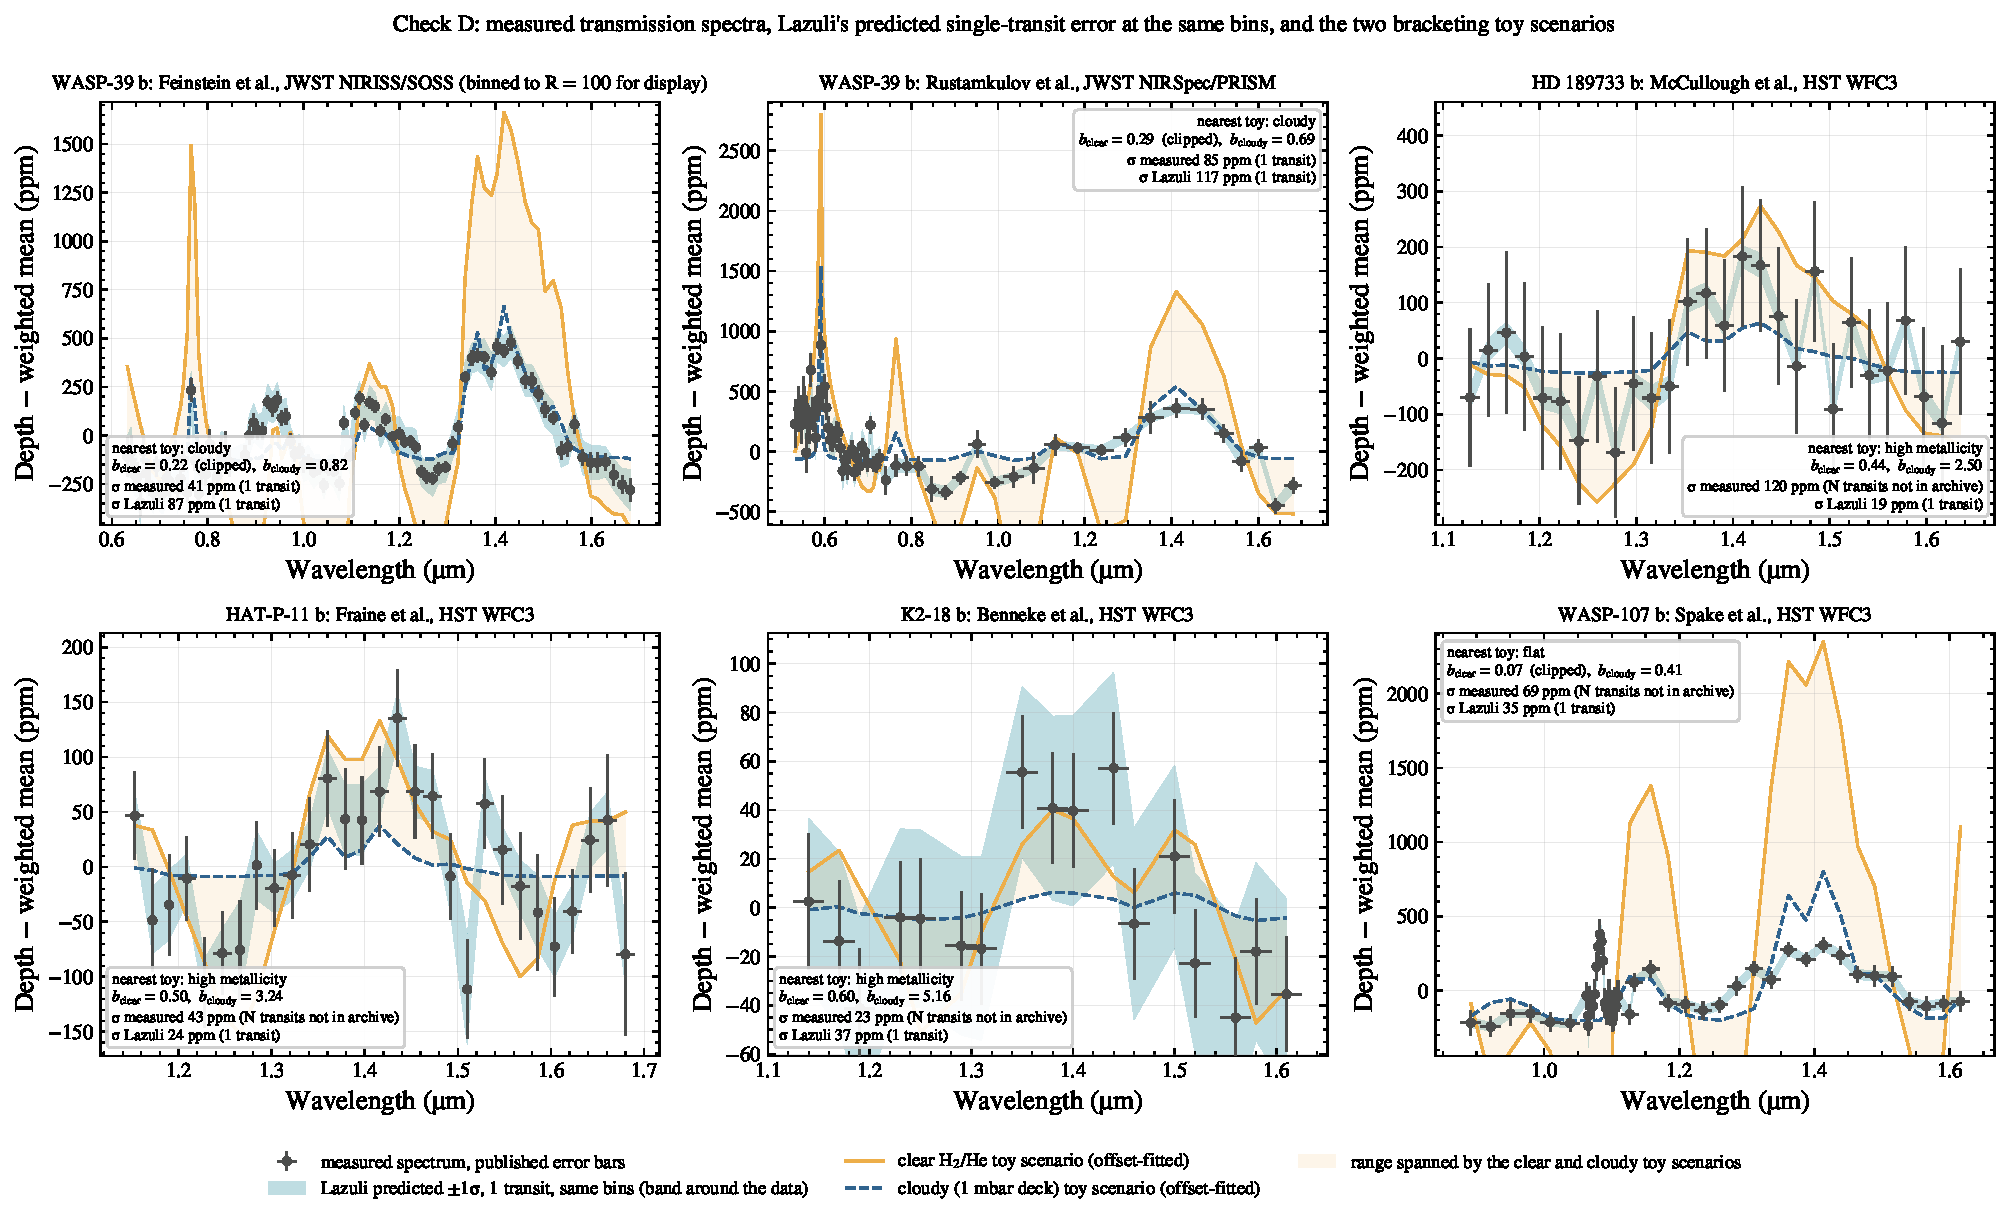
\includegraphics[width=\textwidth]{figures/checkD_spectra.pdf}
\caption*{\footnotesize\textbf{Figure 3.} Six measured transmission spectra (gray circles, published error bars and bin widths; the weighted mean depth is subtracted) with Lazuli's predicted single-transit $\pm1\sigma$ at the same bins drawn as a teal band around the data, and the two bracketing toy scenarios from the POSEIDON tables, offset-fitted and binned to the same bins: clear H$_2$/He (amber) and cloudy, 1\,mbar deck (blue dashed), with the range between them shaded. The y-range follows the data and the cloudy model; where the clear model leaves it the box says ``clipped'' and gives its amplitude ratio $b_{\rm clear}$. Each box also gives the nearest toy scenario, $b_{\rm cloudy}$, the median published error with the number of transits it combines (1 for the two JWST ERS spectra; not recorded in the archive for HST), and Lazuli's median predicted single-transit error. The NIRISS/SOSS spectrum is binned to $R=100$ for display only; its table entries use the native bins. Derived here; data from the NASA Exoplanet Archive.}
\end{figure}

The clear H$_2$/He scenario over-predicts the measured feature amplitude everywhere: $b_{\rm clear}\le0.69$ for all 33 space-based datasets with at least ten points, and negative for seven of them (the two WASP-12\,b datasets and five of the six TRAPPIST-1\,e visits, whose structure anti-correlates with the model). The cloudy (1\,mbar) scenario under-predicts most of them, so the set brackets the data for 23 of 47 datasets on the table path and 31 of 47 on the parametric path (15 and 22 of 35 space-based); the parametric path brackets more because its amplitudes are 10--50\,\% smaller (the reference-radius convention, GitHub \#3), not because it is a better model. The nearest toy scenario is consistent with the published interpretations where the data constrain it: high metallicity for K2-18\,b (both WFC3 reductions), HAT-P-11\,b and HD~189733\,b WFC3; cloudy for HD~209458\,b and WASP-39\,b; flat for WASP-107\,b and TRAPPIST-1\,e. This is not model selection: with a free offset and five candidates a nearest label is expected even for a wrong model family, and against JWST-quality data no toy scenario fits ($\chi^2_\nu=5$--$6$ for WASP-39\,b), as expected for isothermal, gray-cloud models. TRAPPIST-1\,e's four JWST visits and two HST visits all have the flat scenario nearest, with $b_{\rm clear}\le0.08$: the H$_2$/He showcase scenarios for this planet are excluded by data, as the published analyses conclude (Espinoza et al.\ 2025). Ground-based datasets with 5--8 points are listed for completeness only; their $b$ values are unconstrained.

\subsection*{G. Stellar contamination}

\begin{table}[H]
\centering\footnotesize
\begin{tabular}{@{}lrrrrrrrrr@{}}
\toprule
\textbf{band ($\mu$m)} & \textbf{$n_\lambda$} & \textbf{$\sigma_{\rm visit}$} & \textbf{std} & \textbf{excess} & \textbf{excess$_{84}$} & \textbf{offsets} & \textbf{Lazuli $\sigma_1$} & \textbf{clear} & \textbf{cloudy} \\
\midrule
0.6-1.0 & 15 & 309 & 287 & 0 & 352 & 431 & 1715 & 2280 & 749 \\
1.0-1.7 & 17 & 126 & 221 & 180 & 237 & 431 & 327 & 3009 & 1306 \\
0.6-1.7 & 32 & 160 & 243 & 168 & 259 & 431 & 396 & 3021 & 1306 \\
\bottomrule
\end{tabular}
\caption*{\footnotesize\textbf{Table G.} Check G, TRAPPIST-1\,e (Espinoza et al.\ 2025, four JWST/NIRSpec PRISM visits, `Espinoza' reduction). All in ppm: median per-visit error; visit-to-visit standard deviation of the depth at each wavelength; the part of it in excess of the per-visit errors (median and 84th percentile); spread of the four visits' weighted-mean depths; lazuli-exo's single-transit error per native channel; and the parametric clear and cloudy H$_2$/He feature amplitudes over the same band. Derived here.}
\end{table}


\begin{figure}[H]
\centering
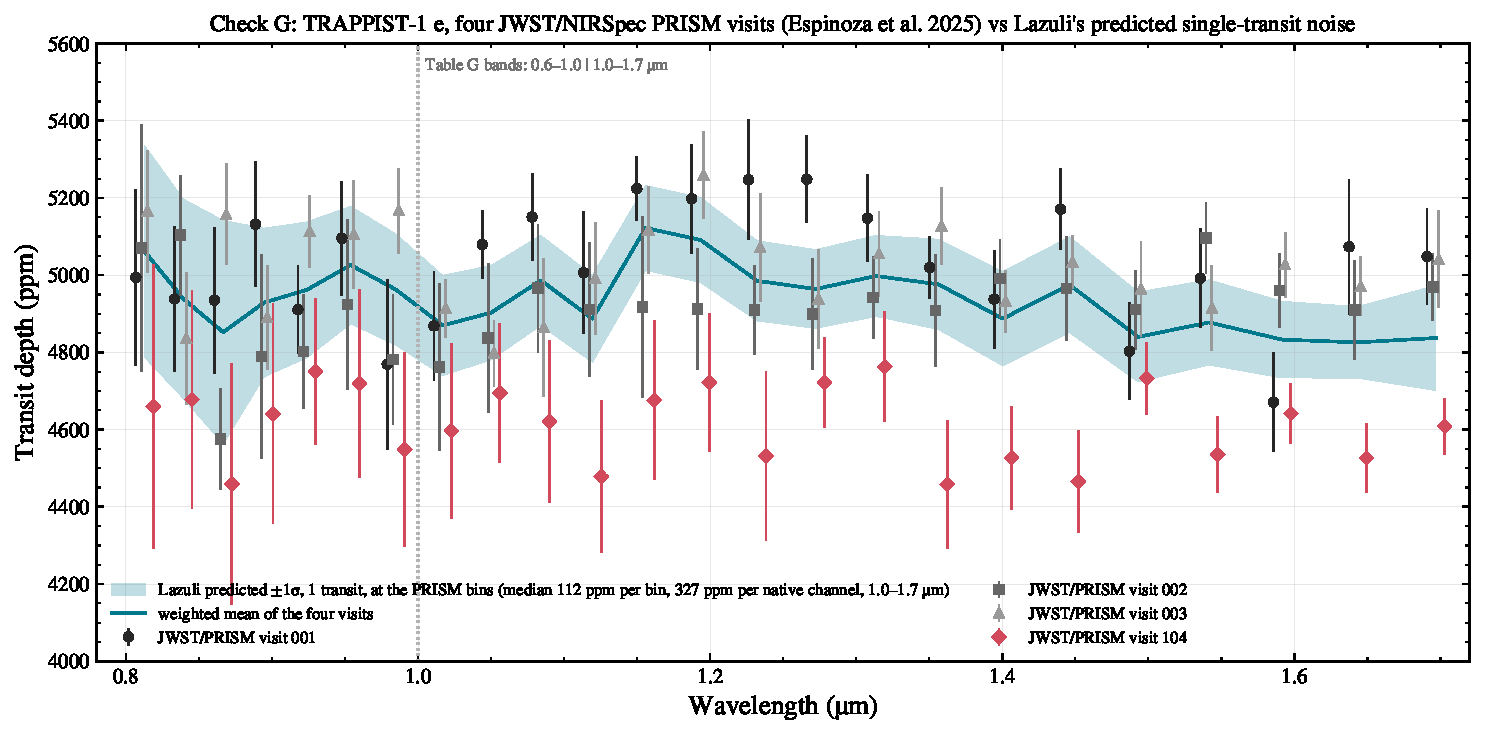
\includegraphics[width=0.85\textwidth]{figures/checkG_trappist1e_visits.pdf}
\caption*{\footnotesize\textbf{Figure 4.} The four JWST/NIRSpec PRISM transmission spectra of TRAPPIST-1\,e from Espinoza et al.\ (2025), `Espinoza' reduction, over 0.8--1.7\,$\mu$m (symbols, published error bars, visits offset slightly in wavelength; the 0.6--0.8\,$\mu$m points have errors of 300--2800\,ppm and are left out of the plot but kept in Table~G), their weighted mean (teal line) and Lazuli's predicted single-transit $\pm1\sigma$ at the same PRISM bins (teal band; median 112\,ppm per bin at 1.0--1.7\,$\mu$m, which is 327\,ppm per native Lazuli channel, Table~G). Visit 104 (red diamonds) sits 300--500\,ppm below the others across the whole band. Derived here from the Zenodo record 16125662 data.}
\end{figure}

At 1.0--1.7\,$\mu$m the four visits scatter by 220\,ppm at fixed wavelength against a median per-visit error of 126\,ppm, leaving 180\,ppm of excess scatter (84th percentile 240\,ppm); the visits' mean depths differ by 430\,ppm. Espinoza et al.\ (2025) attribute this to the transit light source effect and note that current stellar models cannot reproduce it; Lim et al.\ (2023) find for TRAPPIST-1\,b that the stellar-model uncertainty is an order of magnitude above their 89\,ppm precision; Cadieux et al.\ (2024) detect unocculted faculae covering about 20\,\% of LHS~1140 at 5.8$\sigma$. Lazuli's single-transit error for TRAPPIST-1\,e is 330\,ppm per native channel at 1.0--1.7\,$\mu$m (112\,ppm per PRISM-sized bin, Figure~4), so after about three transits the unmodelled stellar term exceeds the statistical one, and it is already larger than the parametric cloudy-scenario amplitude in the blue.

\subsection*{Acceptance criteria}

\begin{table}[H]
\centering\small
\begin{tabularx}{\linewidth}{@{}l p{3.0cm} p{3.6cm} X@{}}
\toprule
\textbf{Check} & \textbf{Measured reference} & \textbf{Pass criterion (v0.1)} & \textbf{Status (v0.2)} \\
\midrule
A & Gaia XP, 2MASS, $V$ & colours within 0.10\,mag; XP within 10\,\% per 50\,nm & pass 7 of 8 hosts with $T_{\rm eff}>4400$\,K (WASP-12 at 1.2 in the blue); fail M dwarfs \\
B(i) & hand photon budget & signal ratio $1.00\pm0.05$ & pass (1.000) \\
B(ii) & achieved HST/JWST precision & $\sigma_{\rm Lazuli}\ge$ scaled photon floor & consistent with JWST; HST indicative \\
C & archive solutions, batman & $t_{14}$ within 2\,\%; residual $<0.2\sigma_{\rm pt}$ & $t_{14}$ fail HAT-P-11\,b, LHS~1140\,b; solver pass; arc fail WASP-12\,b, HAT-P-11\,b, K2-18\,b \\
D & published spectra & scenario set brackets the data & 23/47 (tables), 31/47 (parametric); clear always too large \\
E & fitted LD & $|\Delta I(\mu)|<0.02$ & not run \\
F & H4RG lab ramps & saturation onset within 5\,\% & not run \\
G & JWST M-dwarf epochs & transit-light-source effect (TLSE) bounded before a scenario is added & bounded: 180--430\,ppm for TRAPPIST-1\,e \\
H & slicersim time series & recovered scatter / table $=1.00\pm0.05$ & not run \\
\bottomrule
\end{tabularx}
\caption*{\footnotesize\textbf{Table 3.} Acceptance criteria from v0.1 and the v0.2 outcome.}
\end{table}

% ============================================================================
\section*{Discussion}

\textbf{Limitations.}
\begin{itemize}[leftmargin=*,itemsep=1pt]
  \item Check D cannot validate the toy scenarios; it shows which side of the data they fall on. It does show, with 33 space-based datasets, that ``clear'' is an envelope and never a central estimate.
  \item Check B(ii) inherits each reduction's systematics and the archive does not record how many transits a published spectrum combines. The JWST ratios are the ones to quote; the HST ratios say more about HST than about Lazuli.
  \item The hand budget in B(i) takes $A$, $\eta$ and QE from the same configuration slicersim uses, so it validates units and normalization, not the throughput curve itself. Check F or a measured end-to-end throughput is needed for that.
  \item Gaia XP stops at 1.02\,$\mu$m; the $J{-}H$ colours (within 0.13\,mag for all hosts except GJ~3470 and LHS~1140 on the mini-grid, see Table~A) are the only test of the red half of the band.
  \item Check G uses one reduction of one planet. The TRAPPIST-1 contamination level is extreme; the bound should be redone per host class before it becomes a scenario parameter.
  \item The Lazuli CBE throughput encoded in the noise tables may carry an export classification; the scaled JWST numbers stay internal until that is cleared.
\end{itemize}

\textbf{Implications.} The noise model's normalization is now trustworthy and its photon floor is consistent with what JWST achieves per unit collecting area. The remaining errors are in the inputs and in presentation: an M-dwarf stellar grid that is wrong by tens of percent in the blue, a registry with two inconsistent durations and percent-level ambiguity in $k$, a default ``clear'' scenario that no measured planet reaches, and no stellar-contamination term for the hosts where it dominates. None of these is a code bug in the sense of the 2026-10-05 review; all of them change the numbers a user would quote.

\textbf{Recommendations.}
\begin{enumerate}[leftmargin=*,itemsep=1pt]
  \item Fix the PHOENIX mini-grid (\#16) and, for the showcase M dwarfs, normalize the star to Gaia XP over 0.40--1.02\,$\mu$m rather than to $J$ alone.
  \item Make ``cloudy'' or ``high metallicity'' the default showcase scenario for sub-Neptunes and label ``clear'' as an upper envelope in the UI and docs; remove the H$_2$/He scenarios for TRAPPIST-1\,e and LHS~1140\,b or show them only with the check-D verdict attached (\#8).
  \item Resolve the two-path convention (\#3) before any public number; the bracketing statistics above differ between paths for that reason alone.
  \item Freeze one solution per target with references and uncertainties (\#7); HAT-P-11\,b and LHS~1140\,b first. Constrain the TRAPPIST-1\,e limb-darkening fit so no chunk has negative limb intensity (\#10).
  \item Add a user-settable stellar-contamination term, defaulting to the check-G bound for late-M hosts, and a systematics floor informed by the JWST achieved-to-predicted ratios (\#8).
  \item Run checks E, F and H when fitted LD coefficients, H4RG lab data and slicersim time series become available; wire \texttt{memo/scripts/} into CI so the tables regenerate with every table change.
\end{enumerate}

% ============================================================================
\section*{Appendix}

\textbf{Reproduction.} From the repository root in the \texttt{py313} environment:
\begin{itemize}[leftmargin=*,itemsep=1pt]
  \item \texttt{python memo/scripts/fetch\_data.py} (network): archive spectra and solutions, SIMBAD photometry, Gaia XP, TRAPPIST-1\,e Zenodo files $\rightarrow$ \texttt{memo/data/}.
  \item \texttt{python memo/scripts/checkA\_sed.py}, \texttt{checkB\_photon.py} (needs slicersim), \texttt{checkC\_geometry.py} (needs batman), \texttt{checkD\_spectra.py}, \texttt{checkG\_tlse.py} $\rightarrow$ \texttt{memo/results/*.csv}, \texttt{memo/figures/}.
  \item \texttt{python memo/scripts/make\_tables.py} and \texttt{make\_figures.py} $\rightarrow$ \texttt{memo/results/table\_*.tex} and \texttt{memo/figures/}, which this document inputs.
  \item The v0.1 pilot scripts (\texttt{vegacheck.py}, \texttt{combined.py}, \texttt{satcheck.py}, \texttt{sedcheck.py}, \texttt{physcheck.py}, \texttt{lsfcheck.py}, \texttt{transitcheck.py}) were ported to the \texttt{lazuli\_exo} name and are superseded by the check scripts above.
\end{itemize}

\textbf{Table D2: check D on the parametric path.} Same datasets and columns as Table~D1, with the parametric model at the showcase presets.

\begin{table}[H]
\centering\scriptsize
\begin{tabular}{@{}lllrrrlrrrrl@{}}
\toprule
\textbf{Planet} & \textbf{Dataset} & \textbf{Facility} & \textbf{$n$} & \textbf{amp} & \textbf{$\sigma$} & \textbf{nearest toy} & \textbf{$\chi^2_\nu$} & \textbf{$\chi^2_{\nu,\rm flat}$} & \textbf{$b_{\rm clear}$} & \textbf{$b_{\rm cloudy}$} & \textbf{bracketed} \\
\midrule
GJ 1214 b & Bean et al. 2011, MMIRS & ground & 36 & 1032 & 175 & flat & 1.3 & 1.3 & -0.07 & -0.00 & no \\
GJ 1214 b & Berta et al. 2012, WFC3 & HST & 24 & 778 & 212 & cloudy & 0.6 & 0.8 & 0.22 & 2.32 & yes \\
GJ 1214 b & Croll et al. 2011, WIRCam & ground & 5 & 780 & 340 & high-met & 0.8 & 0.9 & 0.33 & 2.66 & yes \\
GJ 1214 b & Kreidberg et al. 2014, WFC3 & HST & 22 & 99 & 28 & flat & 1.0 & 1.0 & 0.02 & 0.16 & no \\
GJ 1214 b & Rackham et al. 2017, IMACS & ground & 14 & 619 & 185 & flat & 0.8 & 0.8 & -0.23 & -7.57 & no \\
GJ 1214 b & Wilson et al. 2014, OSIRIS & ground & 8 & 2299 & 423 & clear & 4.0 & 4.4 & 1.20 & 119.41 & yes \\
GJ 3470 b & Benneke et al. 2019, STIS & HST & 8 & 303 & 101 & cloudy & 1.2 & 1.2 & 0.17 & 1.86 & yes \\
GJ 3470 b & Benneke et al. 2019, WFC3 & HST & 18 & 161 & 32 & cloudy & 1.6 & 2.3 & 0.11 & 0.95 & no \\
GJ 3470 b & Biddle et al. 2014,  & ground & 8 & 1536 & 291 & hazy & 1.0 & 1.3 & 3.81 & -140.76 & yes \\
GJ 3470 b & Biddle et al. 2014, SBIG & ground & 5 & 596 & 402 & hazy & 0.4 & 0.8 & 4.19 & -38.78 & yes \\
GJ 3470 b & Dragomir et al. 2015, SBIG & ground & 7 & 1492 & 476 & hazy & 0.7 & 0.9 & -1.16 & 229.20 & yes \\
GJ 3470 b & Ehrenreich et al. 2014, WFC3 & HST & 107 & 2598 & 398 & cloudy & 1.4 & 1.4 & 0.26 & 1.40 & yes \\
HAT-P-11 b & Fraine et al. 2014, WFC3 & HST & 29 & 247 & 43 & high-met & 0.9 & 2.0 & 0.58 & 5.18 & yes \\
HD 189733 b & Barnes et al. 2016, HARPS Echelle Spe & ground & 5 & 4500 & 1100 & -- & 2.6 & 2.6 & -- & -- & -- \\
HD 189733 b & Borsa et al. 2016, HARPS Echelle Spe & ground & 7 & 676 & 149 & hazy & 0.8 & 1.9 & -0.90 & 1.32 & yes \\
HD 189733 b & Di Gloria et al. 2015, HARPS Echelle Spe & ground & 6 & 1152 & 365 & hazy & 0.9 & 1.1 & -2.56 & -13.45 & yes \\
HD 189733 b & McCullough et al. 2014, WFC3 & HST & 28 & 352 & 120 & high-met & 0.3 & 0.6 & 0.46 & 3.12 & yes \\
HD 189733 b & Pont et al. 2013, ACS & HST & 10 & 461 & 39 & hazy & 1.3 & 6.5 & 0.66 & 6.07 & yes \\
HD 189733 b & Pont et al. 2013, NICMOS & HST & 6 & 1051 & 246 & flat & 2.8 & 2.8 & -2.26 & -20.39 & no \\
HD 189733 b & Pont et al. 2013, STIS & HST & 12 & 401 & 70 & hazy & 4.0 & 4.5 & 0.03 & 0.59 & no \\
HD 189733 b & Sing et al. 2016, STIS & HST & 18 & 643 & 41 & hazy & 3.6 & 18.8 & 0.50 & 1.79 & yes \\
HD 189733 b & Sing et al. 2016, WFC3 & HST & 29 & 353 & 68 & high-met & 1.1 & 1.9 & 0.46 & 3.07 & yes \\
HD 209458 b & Deming et al. 2013, WFC3 & HST & 28 & 276 & 35 & cloudy & 2.1 & 5.9 & 0.35 & 1.48 & yes \\
HD 209458 b & Sing et al. 2016, STIS & HST & 81 & 701 & 85 & cloudy & 1.9 & 2.0 & 0.36 & 2.32 & yes \\
HD 209458 b & Sing et al. 2016, WFC3 & HST & 29 & 262 & 34 & cloudy & 2.5 & 5.1 & 0.29 & 1.07 & yes \\
K2-18 b & Benneke et al. 2019, WFC3 & HST & 17 & 102 & 23 & high-met & 1.2 & 1.9 & 0.69 & 7.91 & yes \\
K2-18 b & Tsiaras et al. 2019, WFC3 & HST & 17 & 115 & 24 & high-met & 1.1 & 1.6 & 0.50 & 6.73 & yes \\
WASP-107 b & Kreidberg et al. 2018, WFC3 & HST & 20 & 433 & 57 & cloudy & 2.0 & 6.5 & 0.12 & 0.76 & no \\
WASP-107 b & Spake et al. 2018, WFC3 & HST & 49 & 623 & 69 & cloudy & 3.5 & 6.1 & 0.09 & 0.80 & no \\
WASP-12 b & Kreidberg et al. 2015, WFC3 & HST & 13 & 273 & 51 & cloudy & 3.2 & 4.0 & 0.26 & 6.10 & yes \\
WASP-12 b & Mandell et al. 2013, WFC3 & HST & 19 & 646 & 229 & hazy & 0.4 & 0.6 & 0.79 & 8.96 & yes \\
WASP-12 b & Sing et al. 2013, STIS & HST & 20 & 569 & 125 & flat & 1.8 & 1.8 & -0.39 & -6.52 & no \\
WASP-12 b & Stevenson et al. 2014, WFC3 & HST & 29 & 1170 & 100 & flat & 7.6 & 7.6 & -0.67 & -14.39 & no \\
WASP-121 b & Evans et al. 2016, WFC3 & HST & 31 & 1388 & 87 & cloudy & 4.0 & 4.2 & 0.10 & 1.22 & yes \\
WASP-39 b & Feinstein et al. 2022, NIRISS & JWST & 213 & 982 & 60 & cloudy & 5.9 & 13.1 & 0.28 & 1.38 & yes \\
WASP-39 b & Fischer et al. 2016, STIS & HST & 31 & 2067 & 263 & cloudy & 1.0 & 1.1 & 0.37 & 2.09 & yes \\
WASP-39 b & Nikolov et al. 2016, FORS2 & ground & 28 & 2017 & 327 & cloudy & 0.7 & 1.2 & 0.47 & 1.31 & yes \\
WASP-39 b & Rustamkulov et al. 2022, Near Infrared Spe & JWST & 63 & 1337 & 85 & cloudy & 5.9 & 8.3 & 0.37 & 1.10 & yes \\
WASP-39 b & Sing et al. 2016, STIS & HST & 31 & 2122 & 281 & cloudy & 1.8 & 1.9 & 0.33 & 2.95 & yes \\
WASP-39 b & Wakeford et al. 2018, WFC3 & HST & 36 & 1128 & 172 & cloudy & 3.6 & 6.0 & 0.42 & 2.05 & yes \\
WASP-96 b & Nikolov et al. 2018, FORS2 & ground & 48 & 1135 & 221 & clear & 1.0 & 1.5 & 0.89 & 2.45 & yes \\
TRAPPIST-1 e & Espinoza et al. 2025, WFC3 visit 1 & HST & 12 & 600 & 150 & flat & 1.4 & 1.4 & -0.12 & 0.35 & no \\
TRAPPIST-1 e & Espinoza et al. 2025, WFC3 visit 2 & HST & 12 & 690 & 130 & flat & 2.2 & 2.2 & -0.46 & -6.58 & no \\
TRAPPIST-1 e & Espinoza et al. 2025, PRISM visit 0 & JWST & 32 & 2045 & 152 & flat & 1.2 & 1.2 & 0.04 & -0.53 & no \\
TRAPPIST-1 e & Espinoza et al. 2025, PRISM visit 0 & JWST & 32 & 6099 & 167 & cloudy & 0.7 & 0.7 & 0.15 & 1.76 & yes \\
TRAPPIST-1 e & Espinoza et al. 2025, PRISM visit 0 & JWST & 32 & 2115 & 129 & flat & 1.0 & 1.0 & 0.01 & -0.09 & no \\
TRAPPIST-1 e & Espinoza et al. 2025, PRISM visit 1 & JWST & 32 & 3343 & 214 & flat & 0.8 & 0.8 & -0.04 & -0.74 & no \\
\bottomrule
\end{tabular}
\caption*{\footnotesize\textbf{Table D2.} Parametric model with the same showcase presets (appendix; same datasets as Table D1). Check D. Every dataset with $\ge 5$ points and errors inside 0.40--1.70\,$\mu$m (NASA Exoplanet Archive; TRAPPIST-1\,e from Espinoza et al.\ 2025). ``amp'' and $\sigma$: measured peak-to-peak depth and median error (ppm). ``nearest toy'' is the scenario with the lowest offset-fit $\chi^2_\nu$ (also given for the flat scenario); with a free offset and five candidates a nearest label is expected even for a wrong model family, so it is not a detection of that scenario. $b$ is the fitted data/model amplitude ratio (1 = the scenario has the measured amplitude); ``bracketed'' = the four atmospheric scenarios' $b$ values (hazy and high-metallicity in \texttt{checkD\_spectra\_summary.csv}) straddle 1. Derived here.}
\end{table}


\textbf{Data sources (accessed 2026-10-05).}
\begin{itemize}[leftmargin=*,itemsep=0pt]\small
  \item NASA Exoplanet Archive, Transmission Spectroscopy table (\texttt{transitspec}) and Planetary Systems table (\texttt{ps}), TAP service, \url{https://exoplanetarchive.ipac.caltech.edu}. The per-dataset reference strings in Tables~B2, D1 and D2 are the archive's own; depths are in percent there and converted here.
  \item Gaia DR3 XP\_SAMPLED spectra via the ESA Gaia archive (astroquery); SIMBAD photometry via astroquery.
  \item Espinoza et al.\ (2025) data and software, Zenodo record 16125662, \url{https://zenodo.org/records/16125662} (files \texttt{appendix-figure1/spectra/JWST\_PRISM\_Espinoza*.txt}, \texttt{HST\_WFC3IR\_visit*.txt}).
  \item slicersim 1.0.0 (\texttt{0947b53}, 2026-09-17), configuration \texttt{lazuli\_cbe.toml}: $A=7.07$\,m$^2$, $\eta(\lambda)$, QE$(\lambda)$, $t_{\rm frame}=2.83$\,s.
\end{itemize}

\textbf{References: data used in checks D and G (verified against arXiv abstracts on 2026-10-05).}
\begin{itemize}[leftmargin=*,itemsep=0pt]\small
  \item Cadieux, C., Doyon, R., MacDonald, R.~J., et al.\ 2024, ApJL 970, L2, ``Transmission Spectroscopy of the Habitable Zone Exoplanet LHS~1140\,b with JWST/NIRISS'', \url{https://arxiv.org/abs/2406.15136}. Source of the faculae result quoted in check G.
  \item Espinoza, N., Allen, N.~H., Glidden, A., et al.\ 2025, ApJL 990, L52, ``JWST-TST DREAMS: NIRSpec/PRISM Transmission Spectroscopy of the Habitable Zone Planet TRAPPIST-1\,e'', \url{https://arxiv.org/abs/2509.05414}. Source of the TRAPPIST-1\,e spectra in checks D and G.
  \item Feinstein, A.~D., Radica, M., Welbanks, L., et al.\ 2023, Nature, ``Early Release Science of the exoplanet WASP-39b with JWST NIRISS'', \url{https://arxiv.org/abs/2211.10493}. NIRISS/SOSS spectrum of WASP-39\,b (archive rows ``Feinstein et al.\ 2022'').
  \item Lim, O., Benneke, B., Doyon, R., et al.\ 2023, ApJL, ``Atmospheric Reconnaissance of TRAPPIST-1\,b with JWST/NIRISS: Evidence for Strong Stellar Contamination in the Transmission Spectra'', \url{https://arxiv.org/abs/2309.07047}. Source of the 89\,ppm precision and the order-of-magnitude stellar-model uncertainty.
  \item Rustamkulov, Z., Sing, D.~K., Mukherjee, S., et al.\ 2023, Nature, ``Early Release Science of the exoplanet WASP-39b with JWST NIRSpec PRISM'', \url{https://arxiv.org/abs/2211.10487}. PRISM spectrum of WASP-39\,b (archive rows ``Rustamkulov et al.\ 2022'').
  \item Sing, D.~K., Fortney, J.~J., Nikolov, N., et al.\ 2016, Nature, ``A continuum from clear to cloudy hot-Jupiter exoplanets without primordial water depletion'', \url{https://arxiv.org/abs/1512.04341}. STIS and WFC3 spectra of HD~189733\,b, HD~209458\,b, WASP-39\,b.
  \item Radica, M., Welbanks, L., Espinoza, N., et al.\ 2023, MNRAS, ``Awesome SOSS: Transmission Spectroscopy of WASP-96b with NIRISS/SOSS'', \url{https://arxiv.org/abs/2305.17001}. Not used: the spectrum is not in the archive and no public data file was located; WASP-96\,b is checked with Nikolov et al.\ (2018) FORS2 data from the archive.
  \item Benneke, B., Roy, P.-A., Coulombe, L.-P., et al.\ 2024, ``JWST Reveals CH$_4$, CO$_2$, and H$_2$O in a Metal-rich Miscible Atmosphere on a Two-Earth-Radius Exoplanet'', \url{https://arxiv.org/abs/2403.03325}. Not used: the TOI-270\,d NIRISS spectrum is not in the archive and no public data file was located.
  \item Other archive datasets in Tables~B2, D1 and D2 (Kreidberg et al.\ 2014, Deming et al.\ 2013, McCullough et al.\ 2014, Fraine et al.\ 2014, Benneke et al.\ 2019, Tsiaras et al.\ 2019, Spake et al.\ 2018, Stevenson et al.\ 2014, Evans et al.\ 2016, Wakeford et al.\ 2018, Nikolov et al.\ 2016, 2018, and others) are cited as the NASA Exoplanet Archive records them; they were not individually re-verified against the papers.
\end{itemize}

\textbf{References: methods and tools (verified).}
\begin{itemize}[leftmargin=*,itemsep=0pt]\small
  \item De Angeli, F., Weiler, M., Montegriffo, P., et al.\ 2023, A\&A, ``Gaia Data Release 3: Processing and validation of BP/RP low-resolution spectral data'', \url{https://arxiv.org/abs/2206.06143}.
  \item Montegriffo, P., De Angeli, F., Andrae, R., et al.\ 2023, A\&A, ``Gaia Data Release 3: External calibration of BP/RP low-resolution spectroscopic data'', \url{https://arxiv.org/abs/2206.06205}.
  \item Rauscher, B.~J., Fox, O., Ferruit, P., et al.\ 2007, PASP, ``Detectors for the James Webb Space Telescope Near-Infrared Spectrograph I: Readout Mode, Noise Model, and Calibration Considerations'', \url{https://arxiv.org/abs/0706.2344}. slicersim's up-the-ramp variance model (Table~B1, last column).
  \item JWST User Documentation, ``JWST Telescope'', \url{https://jwst-docs.stsci.edu/jwst-observatory-hardware/jwst-telescope}: 25.4\,m$^2$ collecting area.
  \item Kreidberg, L.\ 2015, PASP, batman (not re-verified in this draft); Winn, J.~N.\ 2010, transit duration and impact-parameter expressions (not re-verified in this draft).
\end{itemize}

\textbf{Internal, unpublished}
\begin{itemize}[leftmargin=*,itemsep=0pt]\small
  \item \texttt{2026-09-26\_audit\_report.md} and \texttt{report/2026-10-05\_report.md}: the audit and review this memo follows up.
  \item GitHub issues \#3, \#7, \#8, \#12, \#16 at \texttt{schmidt-observatories/lazuli-exo} (private).
\end{itemize}

\end{document}
